\documentclass[aspectratio=43]{beamer}
\usepackage[utf8]{inputenc}
\usepackage{polski}
% \usepackage[polish]{babel}
\usepackage[T1]{fontenc}
\usepackage{tikz}
\usepackage{tikzducks}
% \usetikzlibrary{decorations.pathmorphing}
\usepackage{multimedia}
\usepackage{graphicx}
\usepackage[justification=centering]{caption}
\usepackage{textcomp}
\usepackage{appendixnumberbeamer}
\usepackage{qrcode}
% \usepackage[natbib, language=polish, sorting=none]{biblatex}
% \addbibresource{lio.bib}
\usepackage{hyperref}
%\usepackage[width=\textwidth]{animate}
%\usepackage{chemformula}
\usepackage{sidecap}
\usepackage{multirow}
\usepackage{multicol}
\usepackage{rotating}
\usepackage{anyfontsize} % change font size for semposiwko

% \usepackage{physics}
\usepackage{array}
\usepackage{booktabs}
\usepackage{transparent}
\usepackage{siunitx}
% \usepackage[rightcaption]{sidecap}
\usepackage{eso-pic}

\usepackage{listings}
\lstset{
basicstyle=\small\ttfamily,
columns=flexible,
breaklines=true
}

% \usepackage{emoji}
\usepackage{subcaption}


\usepackage[natbib, language=polish, sorting=none]{biblatex}
\addbibresource{lio.bib}
\renewcommand*{\bibfont}{\scriptsize}

\usefonttheme[onlymath]{serif}

\usetheme{Szeged}
\usecolortheme{whale}
\setbeamercolor{palette primary}{bg=violet!80!black,fg=white}
\setbeamercolor{palette secondary}{bg=violet!60!black,fg=white}
\setbeamercolor{palette tertiary}{bg=violet!40!black,fg=white}
\setbeamercolor{palette quaternary}{bg=violet!20!black,fg=white}
\setbeamercolor{structure}{fg=violet!60!black}
\setbeamertemplate{caption}{\insertcaption}
% \setbeamertemplate{headline}{
%   \begin{beamercolorbox}[wd=.9\paperwidth]{headline}
%     \vspace{1.5ex}
%     \insertsectionnavigationhorizontal
%     \vspace{1.5ex}
%   \end{beamercolorbox}
% }

\linespread{0.6}

\setbeamertemplate{background}%
{%
    \begin{tikzpicture}[remember picture,overlay]{\node[yshift=1.5cm,xshift=-2cm,opacity=0.1] at (current page.south east)
      {
      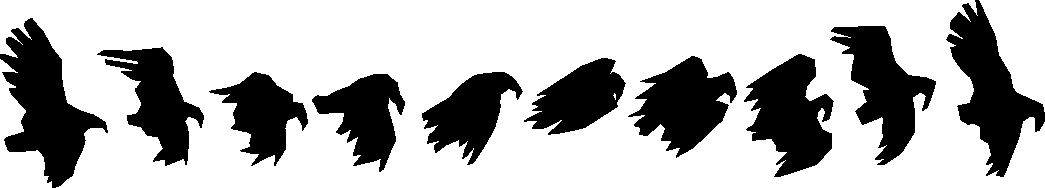
\includegraphics[scale=0.4, angle=20]{ptaki.pdf}
      }
      ;
    \node[yshift=1.0cm,xshift=0.6cm] (logopos) at (current page.south west) {{\begin{tikzpicture}\shuffleducks\duck[signpost=\insertframenumber, \randomhead,scale=.4]\end{tikzpicture}}};
    \pgfmathsetmacro{\progress}{360*(\insertframenumber)/(\inserttotalframenumber)};
    \draw[line width=0.2*3pt] ([xshift=0.55cm] logopos)  arc[radius=0.55cm, start angle=0, end angle=\progress];
    \fill ([shift={(\progress:0.55cm)}] logopos) circle(1pt);

    }
        \end{tikzpicture}
    
}

\newcommand{\SeMPowisko}{%
\large S\normalsize%
\kern-.3em \lower.2ex\hbox{e}%
\lower.2ex\hbox{\large M\normalsize}%
\kern-.1em \raise.1ex\hbox{\large P\normalsize}%
\kern-.3em \lower.2ex\hbox{o}%
\kern-.2em \raise.2ex\hbox{w}%
\lower.2ex\hbox{i}%
s%
\raise.2ex\hbox{k}%
\kern-.3em \lower.2ex\hbox{o}%
}

% \newcommand\Tikz{Ti\emph{k}Z}
% \definecolor{neworange}{RGB}{255,140,0}

\setbeamertemplate{title page}[colsep=-4bp,rounded=true,shadow=true]



\title{Nie oceniaj książki po okładce}
\subtitle{czyli standup o okładkach podręczników do fizyki}
\author[M. Winiarski]{Mateusz ,,\(\blacksquare\)'' Winiarski}
\institute[KMPS UJ]{KMPS UJ \\biofizyka, FAIS, Uniwersytet Jagielloński}
\date[dzisiaj]{TWINK 2025\\dzisiaj}

\begin{document}

\frame{\titlepage}

\section{I semestr}

\subsection{Algebra liniowa z geometrią}

\begin{frame}{Algebra liniowa z geometrią}
\begin{columns}

\column{0.3\textwidth}

\begin{figure}
 \centering
 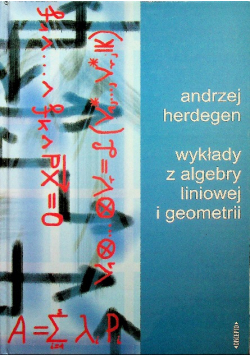
\includegraphics[width=\textwidth]{images/2025-05-09-01-59-23.png}
 \caption{wydanie 1}
 \end{figure}

\column{0.3\textwidth}

\begin{figure}
 \centering
 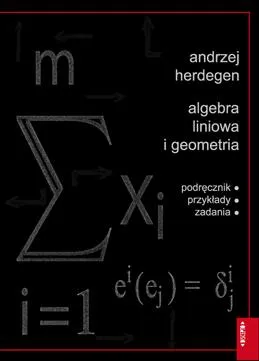
\includegraphics[width=\textwidth]{images/2025-05-09-01-55-59.png}
 \caption{wydanie 2}
 \end{figure}

 \column{0.3\textwidth}

 \begin{figure}
 \centering
 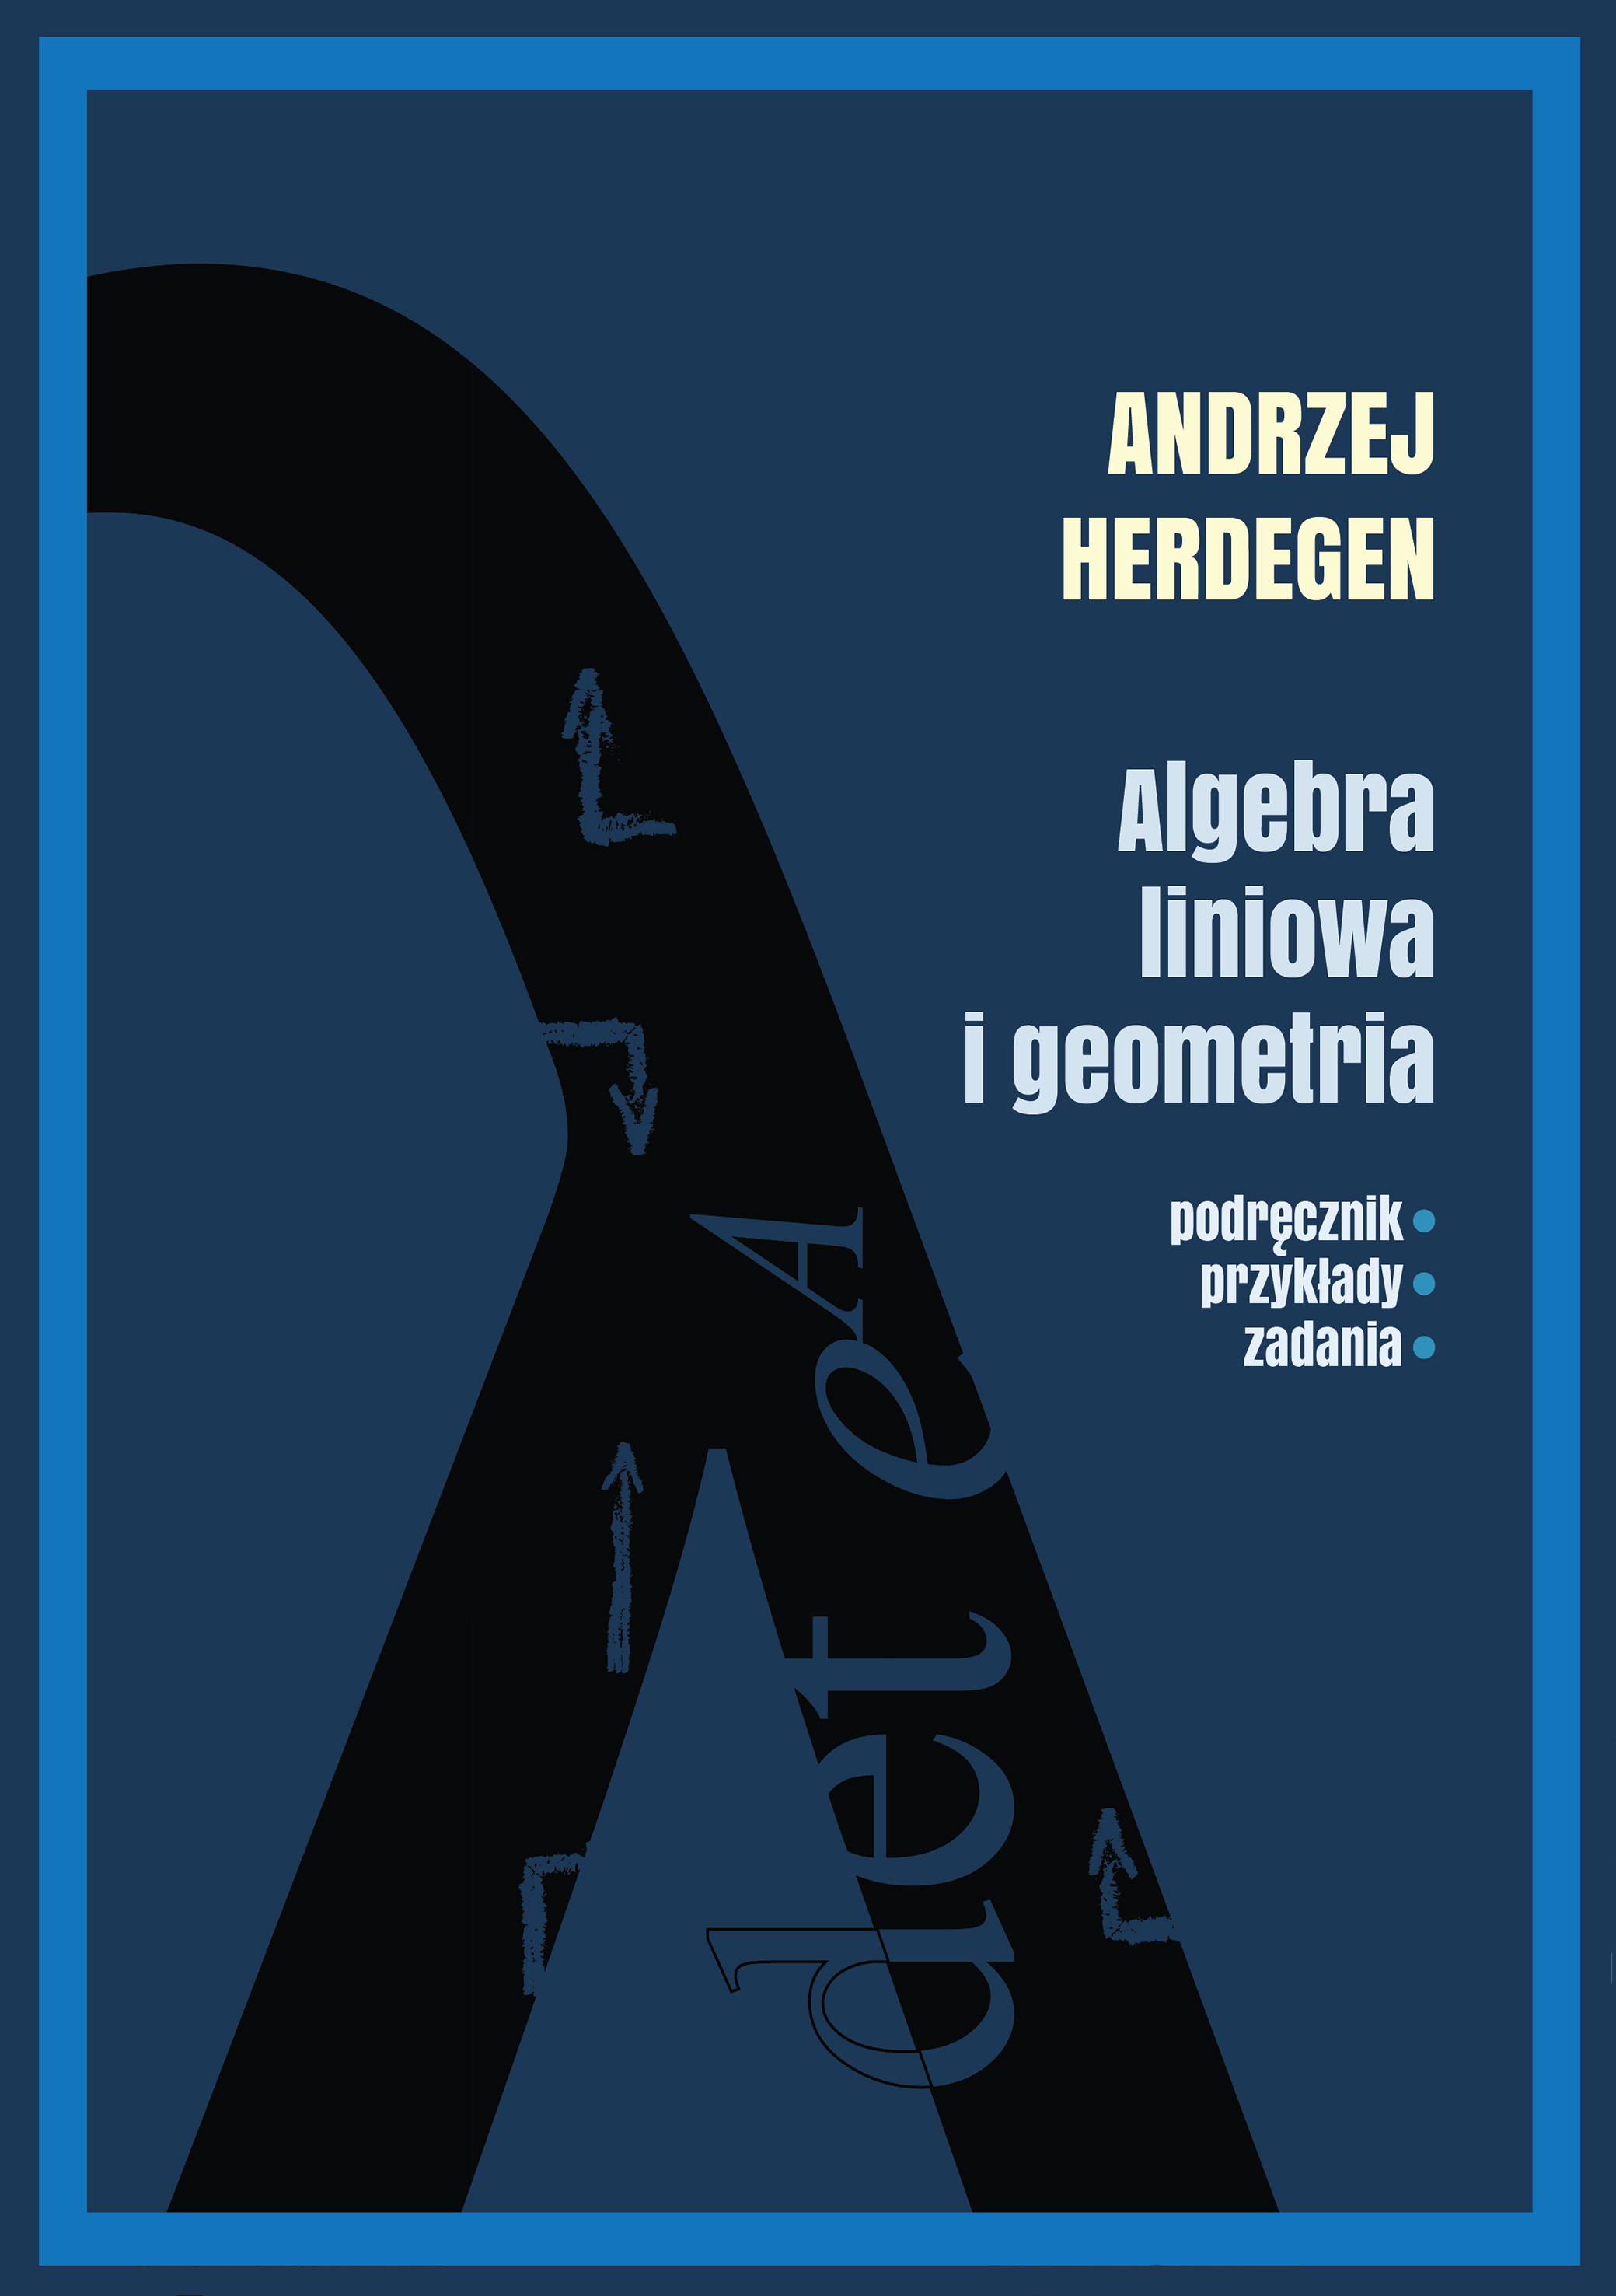
\includegraphics[width=\textwidth]{images/2025-05-09-01-57-53.png}
 \caption{wydanie 3}
 \end{figure}

\end{columns}

\end{frame}

\begin{frame}{Linear Algebra...}
\begin{columns}
\column{0.5\textwidth}
\begin{figure}
 \centering
 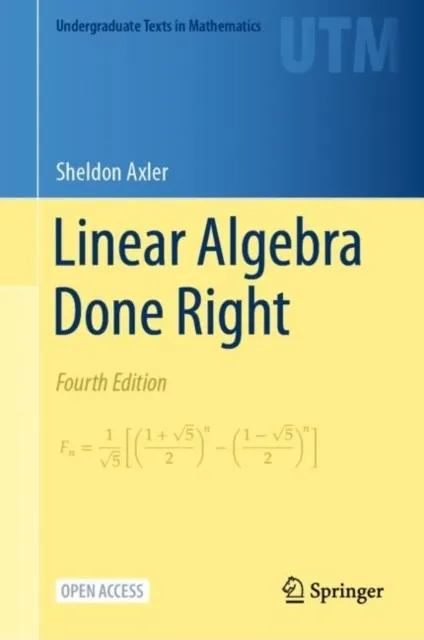
\includegraphics[width=0.7\textwidth]{images/2025-05-16-10-31-17.png}
 \caption{Sheldon Axler, \textit{Linear Algebra Done Right}}
 \end{figure}
\column{0.5\textwidth}\pause
\begin{figure}
 \centering
 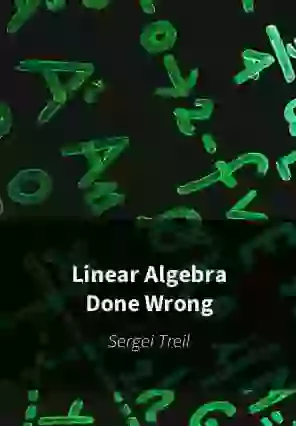
\includegraphics[width=0.7\textwidth]{images/2025-05-16-10-31-53.png}
 \caption{Sergei Treil, \emph{Linear Algebra Done Wrong}}
 \end{figure}
\end{columns}
\end{frame}

\subsection{Analiza matematyczna}
\begin{frame}{Analiza matematyczna w zadaniach}
\begin{columns}
\column{0.5\textwidth}
\begin{figure}
 \centering
 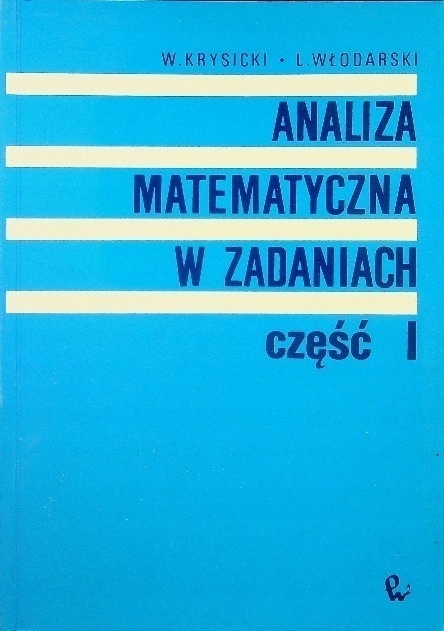
\includegraphics[width=0.7\textwidth]{images/2025-05-19-23-32-14.png}
 \caption{Wydanie nie wiem które}
 \end{figure}

 \column{0.5\textwidth}
\begin{figure}
 \centering
 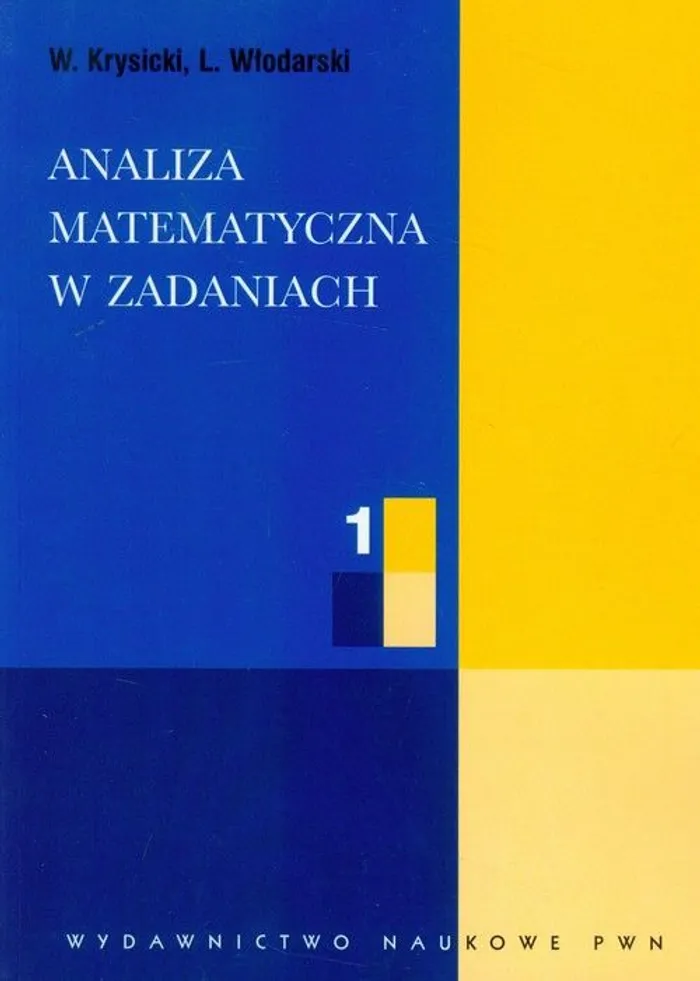
\includegraphics[width=0.7\textwidth]{images/2025-05-19-23-33-11.png}
 \caption{Wydanie pewnie dwudzieste któreś}
 \end{figure}
\end{columns}
\end{frame}

\begin{frame}{Zbiór zadań z analizy matematycznej}
\begin{columns}
\column{0.5\textwidth}
\begin{figure}
 \centering
 
\includegraphics[width=0.7\textwidth]{images/2025-05-19-23-34-13.png}
 \caption{}
 \end{figure}
\column{0.5\textwidth}
\begin{figure}
 \centering
 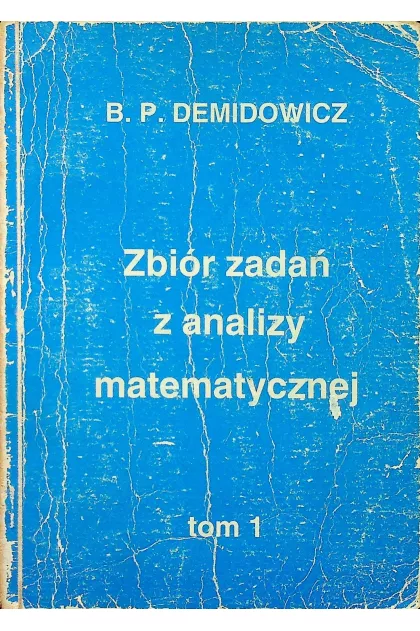
\includegraphics[width=0.7\textwidth]{images/2025-05-19-23-34-47.png}
 \caption{}
 \end{figure}
\end{columns}
\end{frame}

\begin{frame}{Analiza matematyczna}
\begin{figure}
 \centering
 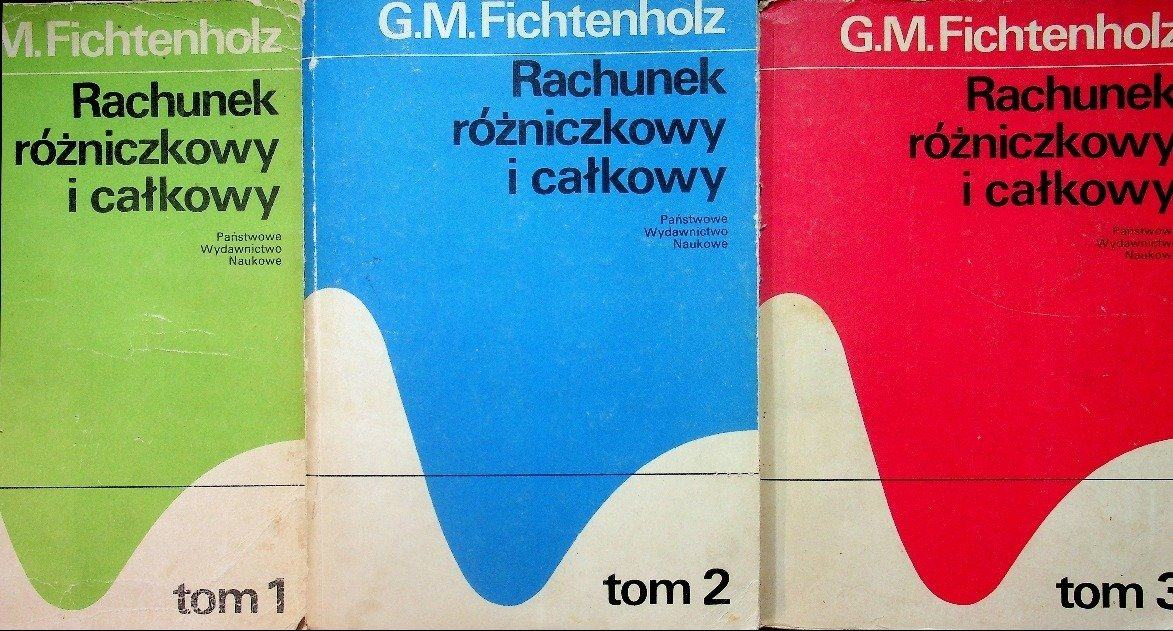
\includegraphics[width=\textwidth]{images/2025-05-19-23-36-44.png}
 \caption{Fichtenholz: trzech nierozłącznych kumpli}
 \end{figure}
\end{frame}

\subsection{Magieranika i inne takie niepotrzebne}
\begin{frame}{Resnick, Halliday, Walker}
  \begin{columns}
  \column{0.5\textwidth}
  \begin{figure}
 \centering
 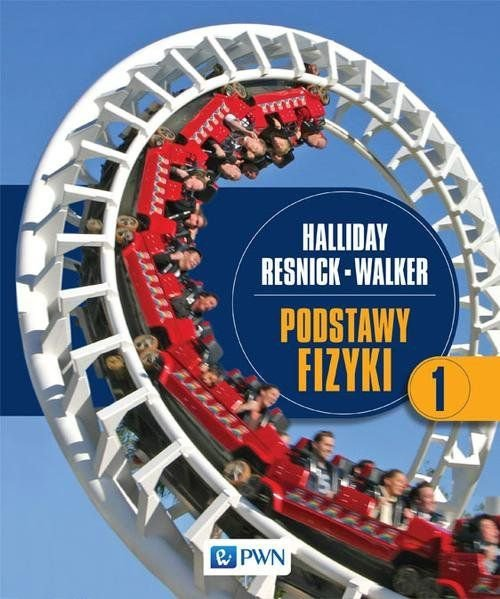
\includegraphics[width=0.5\textwidth]{images/2025-05-19-23-43-04.png}
%  \caption{}
%  \end{figure}
%  \begin{figure}
 \centering
 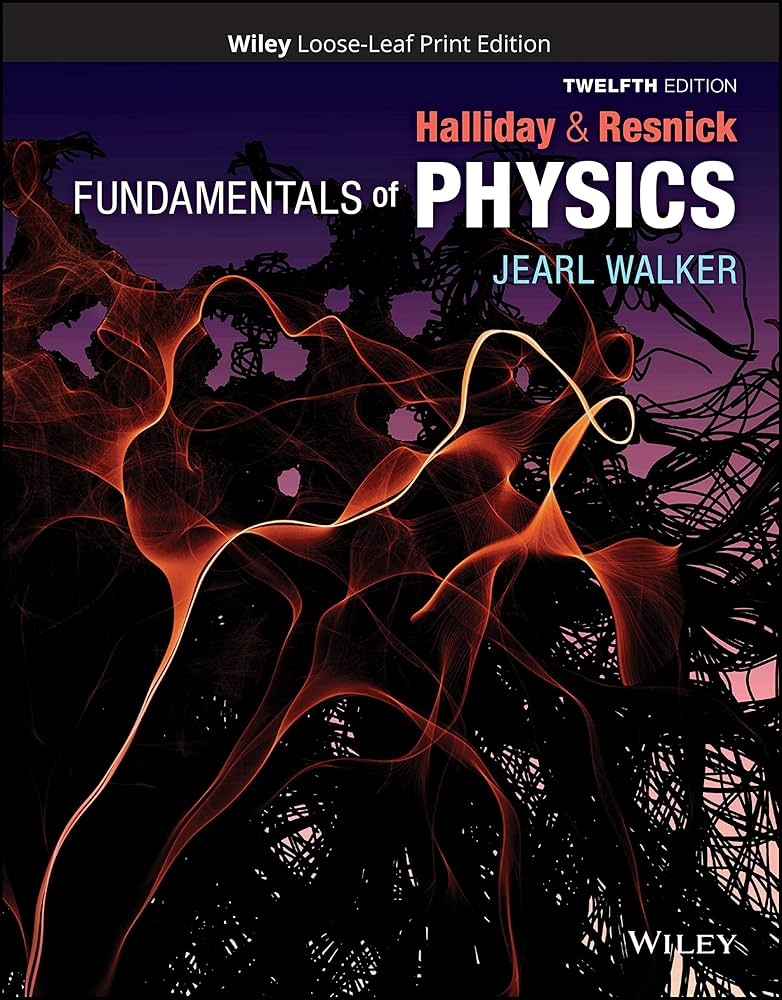
\includegraphics[width=0.5\textwidth]{images/2025-05-20-22-18-44.png}
%  \caption{}
 \end{figure}
  \column{0.5\textwidth}
\begin{figure}
 \centering
 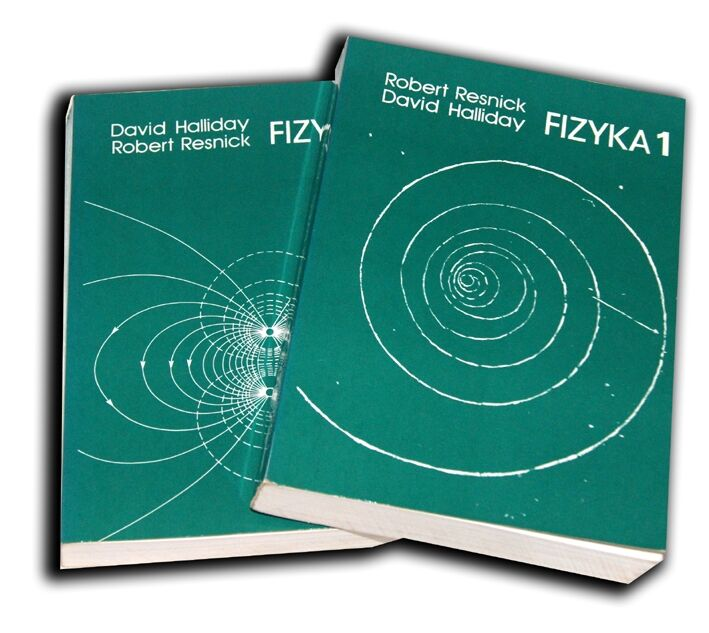
\includegraphics[width=0.6\textwidth]{images/2025-05-20-22-19-27.png}
%  \caption{}
%  \end{figure}
%  \begin{figure}
 \centering
 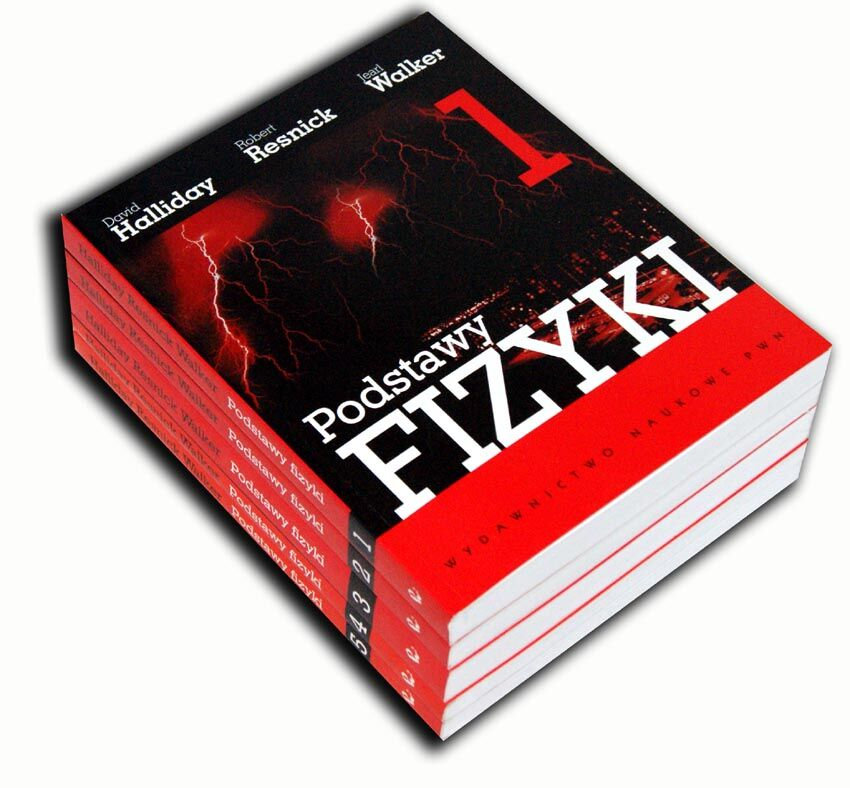
\includegraphics[width=0.6\textwidth]{images/2025-05-20-22-26-46.png}
%  \caption{}
 \end{figure}
\end{columns}

\end{frame}

\begin{frame}{Fajny człowiek (tak naprawdę to nie)}
\begin{columns}
\column{0.5\textwidth}
\begin{figure}
 \centering
 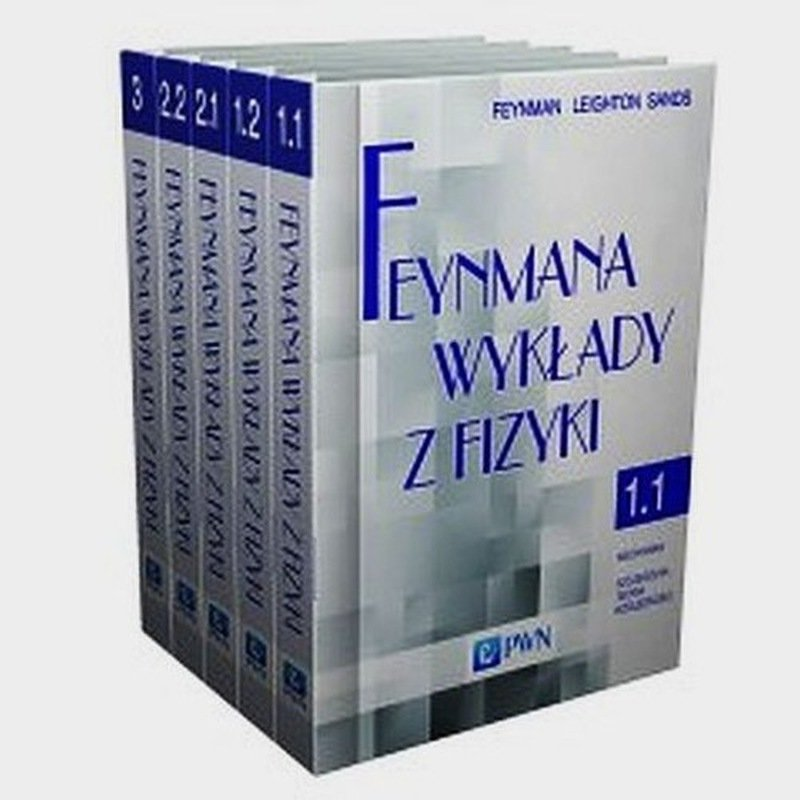
\includegraphics[width=0.5\textwidth]{images/2025-05-20-22-21-07.png}
%  \caption{}
%  \end{figure}
%  \begin{figure}
 \centering
 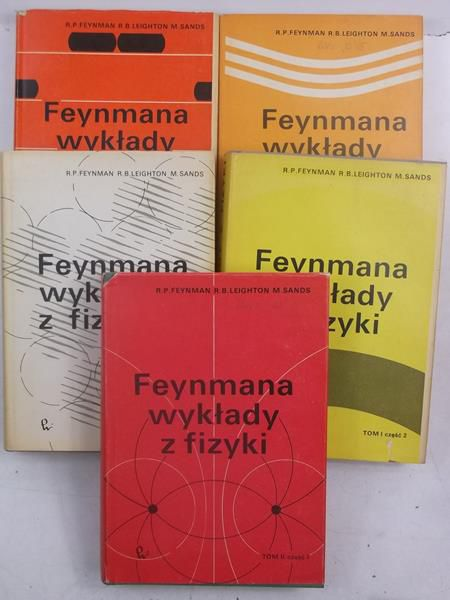
\includegraphics[width=0.5\textwidth]{images/2025-05-20-22-23-09.png}
%  \caption{}
 \end{figure}
 \column{0.5\textwidth}
 \begin{figure}
 \centering
 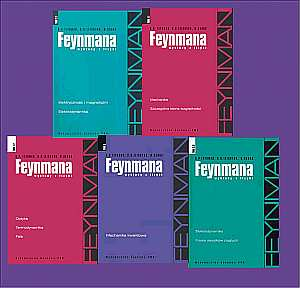
\includegraphics[width=0.6\textwidth]{images/2025-05-20-22-23-42.png}
%  \caption{}
%  \end{figure}
%  \begin{figure}
 \centering
 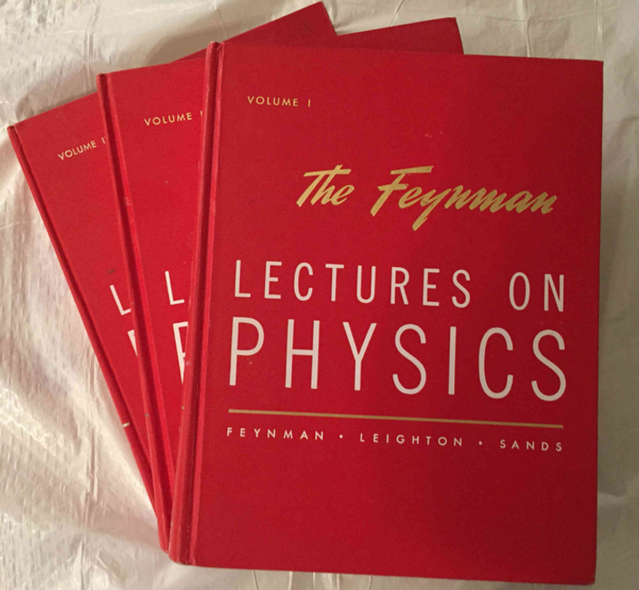
\includegraphics[width=0.6\textwidth]{images/2025-05-20-22-24-15.png}
%  \caption{}
 \end{figure}
  \end{columns}
\end{frame}

\section{II semestr}
\subsection{I pracownia}
\begin{frame}{Magieroskrypt}
  \begin{figure}
 \centering
 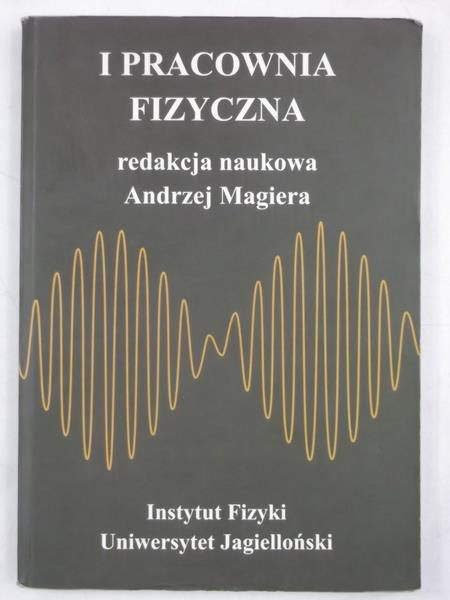
\includegraphics[width=0.5\textwidth]{images/2025-05-20-22-27-47.png}
%  \caption{}
 \end{figure}

\end{frame}

\section{III semestr}
\subsection{Mechanika klasyczna}
\begin{frame}{Mechanika klasyczna}
  \begin{columns}
  \column{0.5\textwidth}

  \begin{figure}
 \centering
 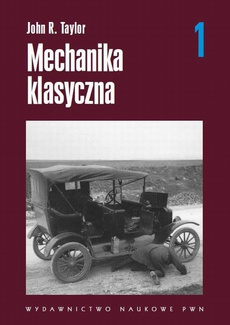
\includegraphics[width=0.7\textwidth]{images/2025-05-20-22-36-55.png}
 \caption{Polak, Anglik, dwa brataniki}
 \end{figure}
\column{0.5\textwidth}
\begin{figure}
 \centering
 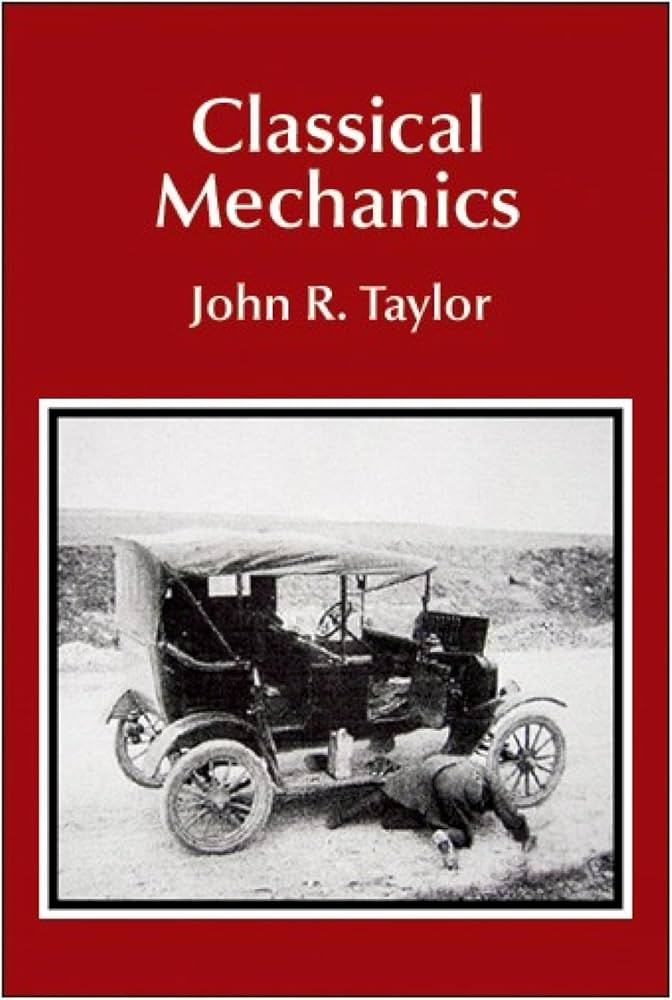
\includegraphics[width=0.7\textwidth]{images/2025-05-20-22-31-52.png}
 \caption{raczej nie nauczą cię mechaniki}
 \end{figure}

 \end{columns}
\end{frame}

\begin{frame}{Mechanika}
  \begin{columns}
    \column{0.3\textwidth}
    \begin{figure}
 \centering
 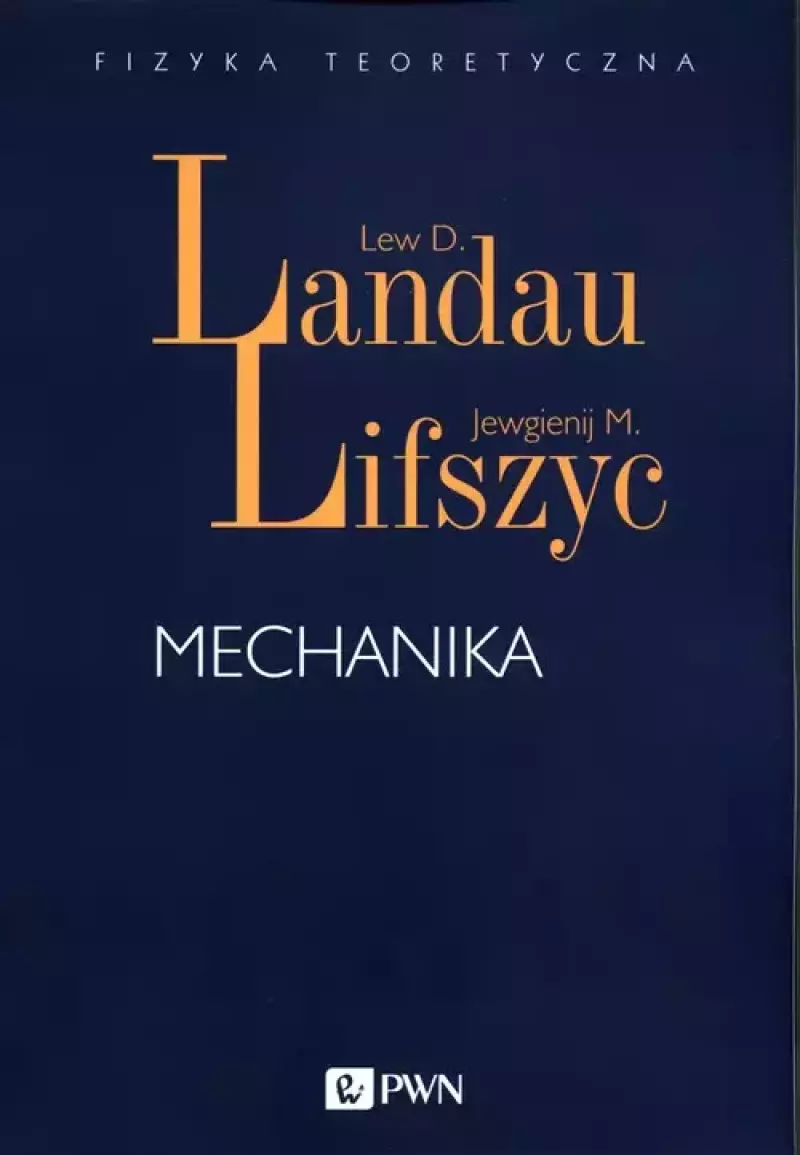
\includegraphics[width=\textwidth]{images/2025-05-20-22-43-27.png}
%  \caption{}
 \end{figure}
 \column{0.3\textwidth}
 \begin{figure}
 \centering
 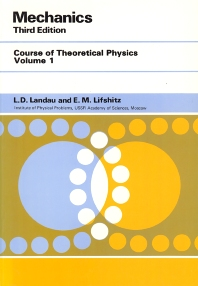
\includegraphics[width=\textwidth]{images/2025-05-20-22-46-04.png}
%  \caption{}
 \end{figure}
 \column{0.3\textwidth}
 \begin{figure}
 \centering
 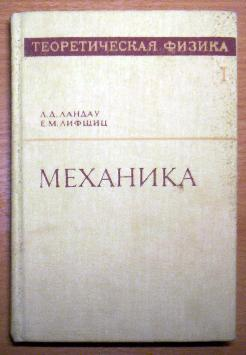
\includegraphics[width=\textwidth]{images/2025-05-20-22-46-50.png}
%  \caption{}
 \end{figure}
  \end{columns}
\end{frame}

\begin{frame}{Metody matematyczne mechaniki klasycznej}
  
% \begin{figure}
  \begin{columns}
    \column{0.3\textwidth}
    \begin{figure}
 \centering
 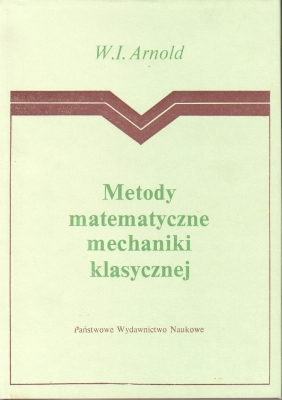
\includegraphics[width=\textwidth]{images/2025-05-20-22-53-16.png}
 \caption{Książka polecana każdemu}
 \end{figure}
    \column{0.3\textwidth}
    \begin{figure}
 \centering
 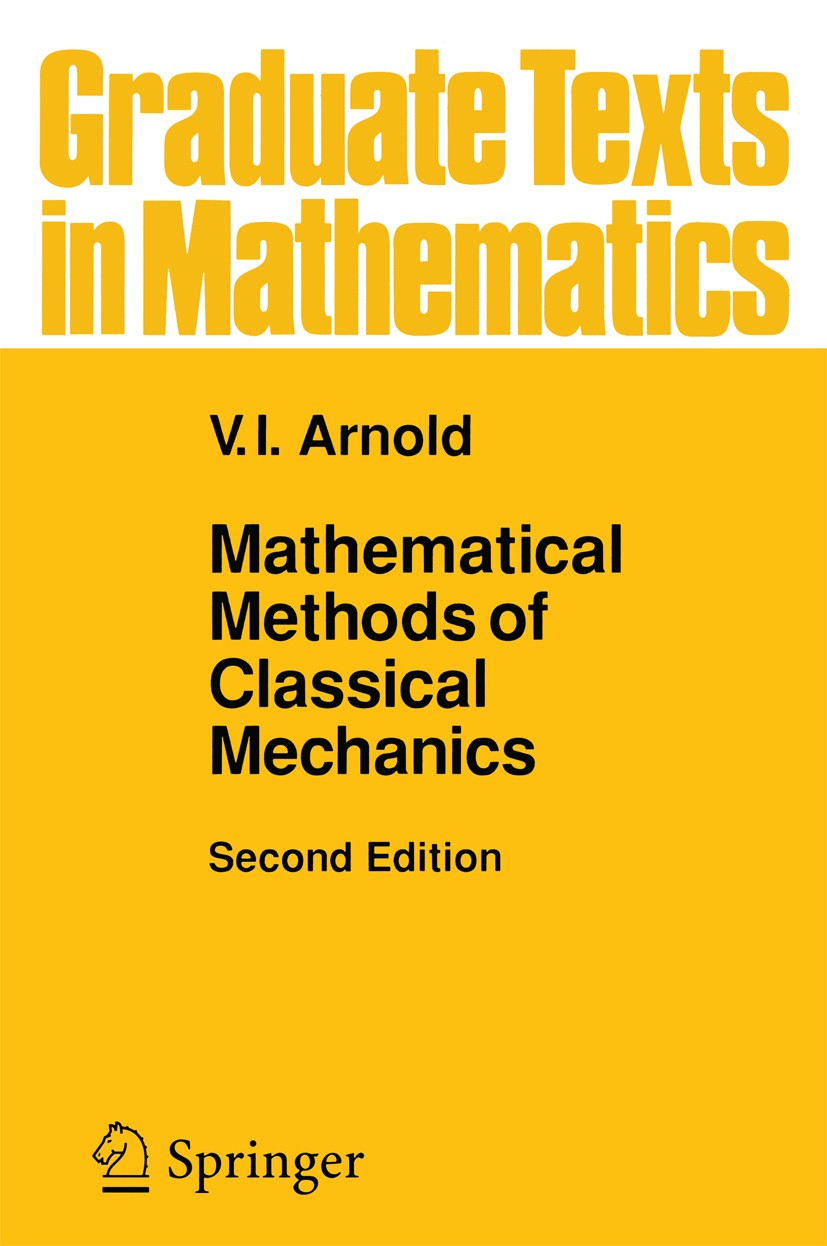
\includegraphics[width=\textwidth]{images/2025-05-20-22-52-51.png}
 \caption{(nie tylko fizykom i matematykom)}
 \end{figure}
    \column{0.3\textwidth}
    \begin{figure}
 \centering
 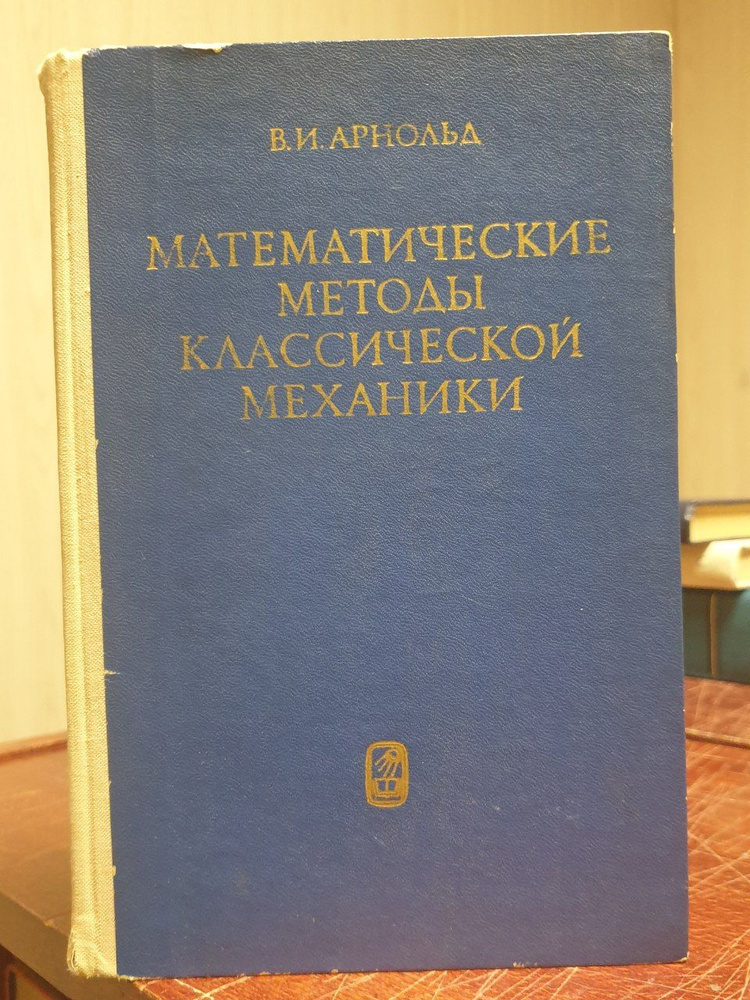
\includegraphics[width=\textwidth]{images/2025-05-20-22-56-11.png}
 \caption{dla niektórych zbyt intuicyjna}
 \end{figure}
  \end{columns}
% \end{figure}
\end{frame}

\subsection{Elektryczność i magnetyzm}  
\begin{frame}{Podstawy elektrodynamiki}
  \begin{columns}
    \column{0.3\textwidth}
\begin{figure}
 \centering
 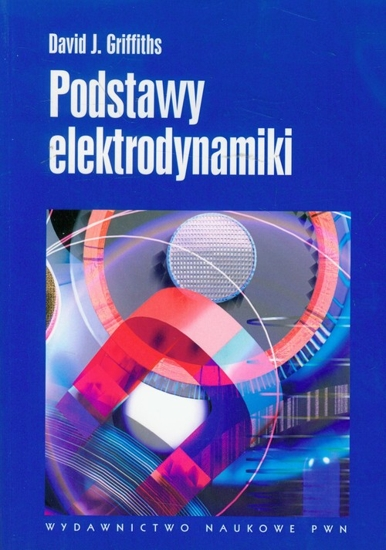
\includegraphics[width=\textwidth]{images/2025-05-20-23-01-23.png}
%  \caption{}
 \end{figure}
 \column{0.3\textwidth}
 \begin{figure}
 \centering
 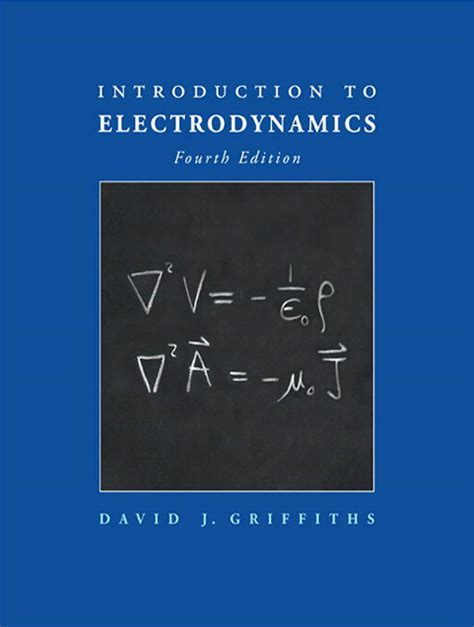
\includegraphics[width=\textwidth]{images/2025-05-20-23-03-10.png}
 \caption{Wydanie IV}
 \end{figure}
 \column{0.3\textwidth}
 \begin{figure}
 \centering
 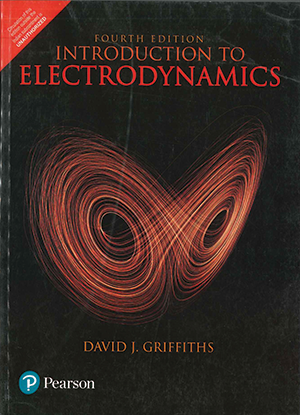
\includegraphics[width=\textwidth]{images/2025-05-20-23-07-47.png}
 \caption{Wydanie IV (???)}
 \end{figure}
  \end{columns}
  
\end{frame}

\section{IV semestr}
\subsection{Mechanika kwantowa}

\begin{frame}{Wstęp do mechaniki kwantowej}
  \begin{columns}
    \column{0.3\textwidth}
    \begin{figure}
 \centering
 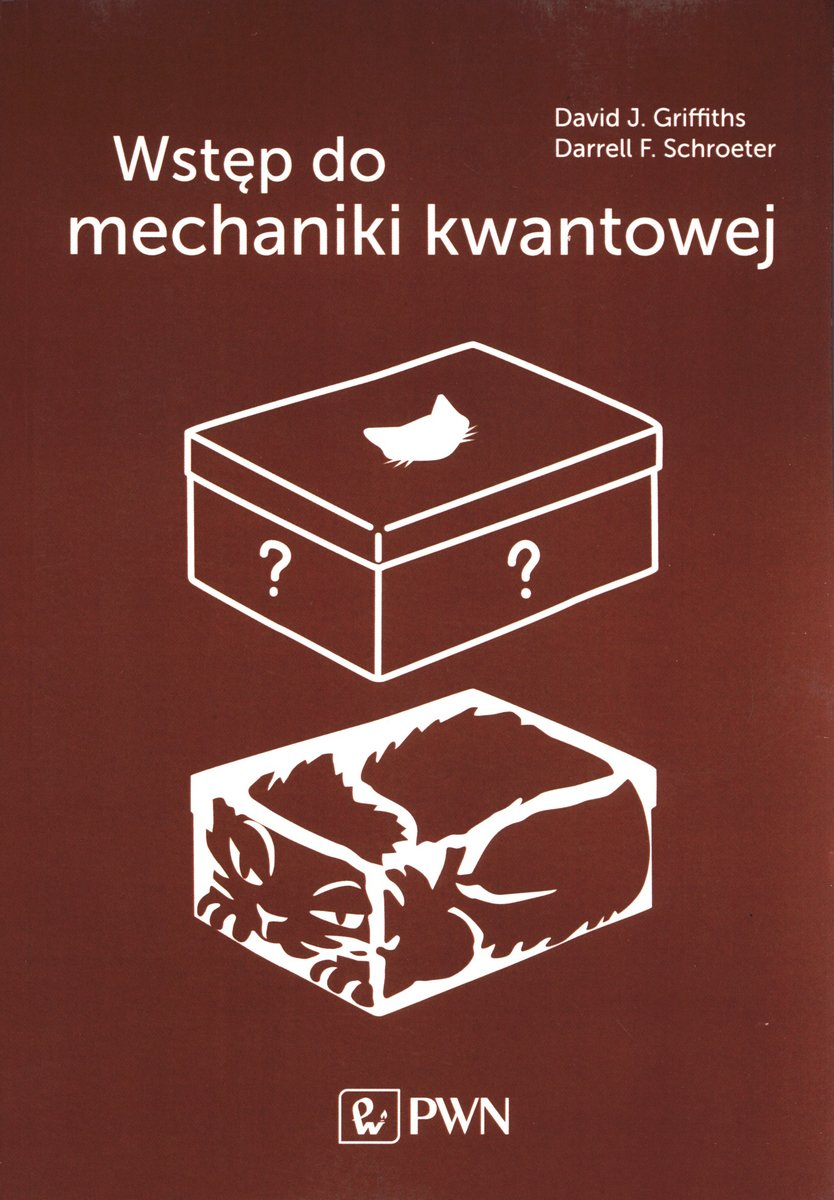
\includegraphics[width=\textwidth]{images/2025-05-20-23-12-27.png}
 \caption{Kotek}
 \end{figure}
 \column{0.3\textwidth}
 \begin{figure}
 \centering
 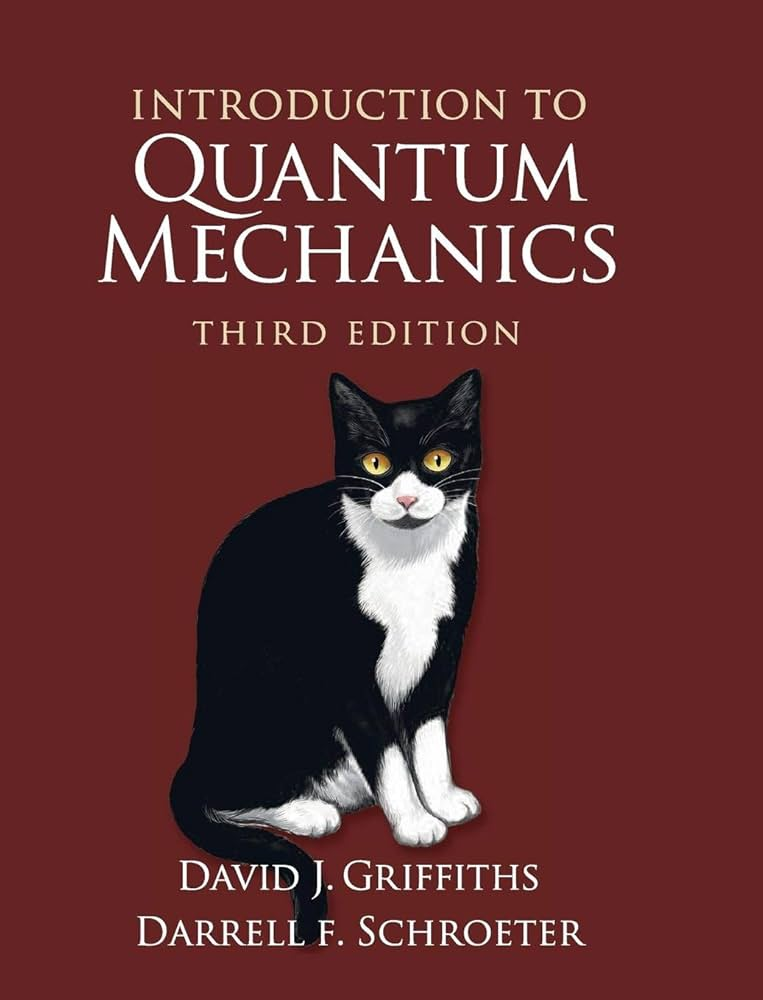
\includegraphics[width=\textwidth]{images/2025-05-20-23-13-22.png}
 \caption{(cat)}
 \end{figure}
 \column{0.3\textwidth}
 \begin{figure}
 \centering
 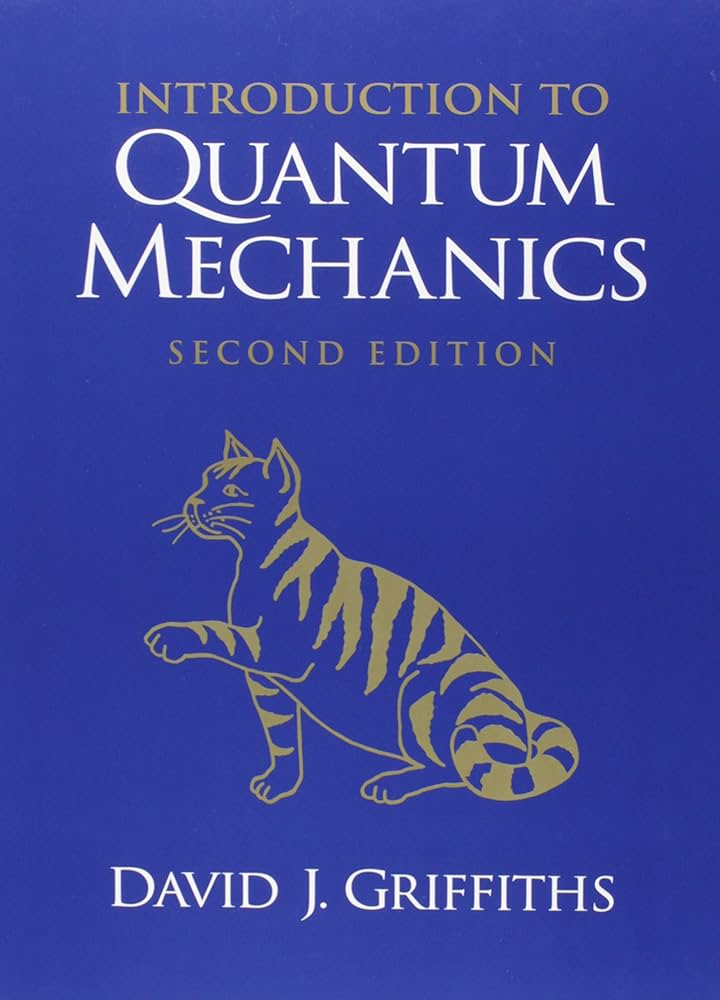
\includegraphics[width=\textwidth]{images/2025-05-20-23-13-58.png}
 \caption{(cat)}
 \end{figure}

 \end{columns}
  
\end{frame}

\begin{frame}{Mechanika kwantowa}
  \begin{columns}
    \column{0.5\textwidth}
 \begin{figure}
 \centering
 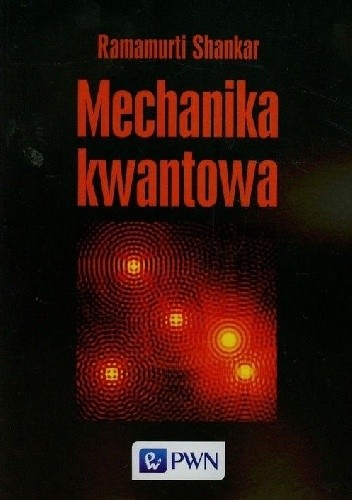
\includegraphics[width=0.8\textwidth]{images/2025-05-20-23-33-33.png}
%  \caption{}
 \end{figure}
  \column{0.5\textwidth}
  \begin{figure}
 \centering
 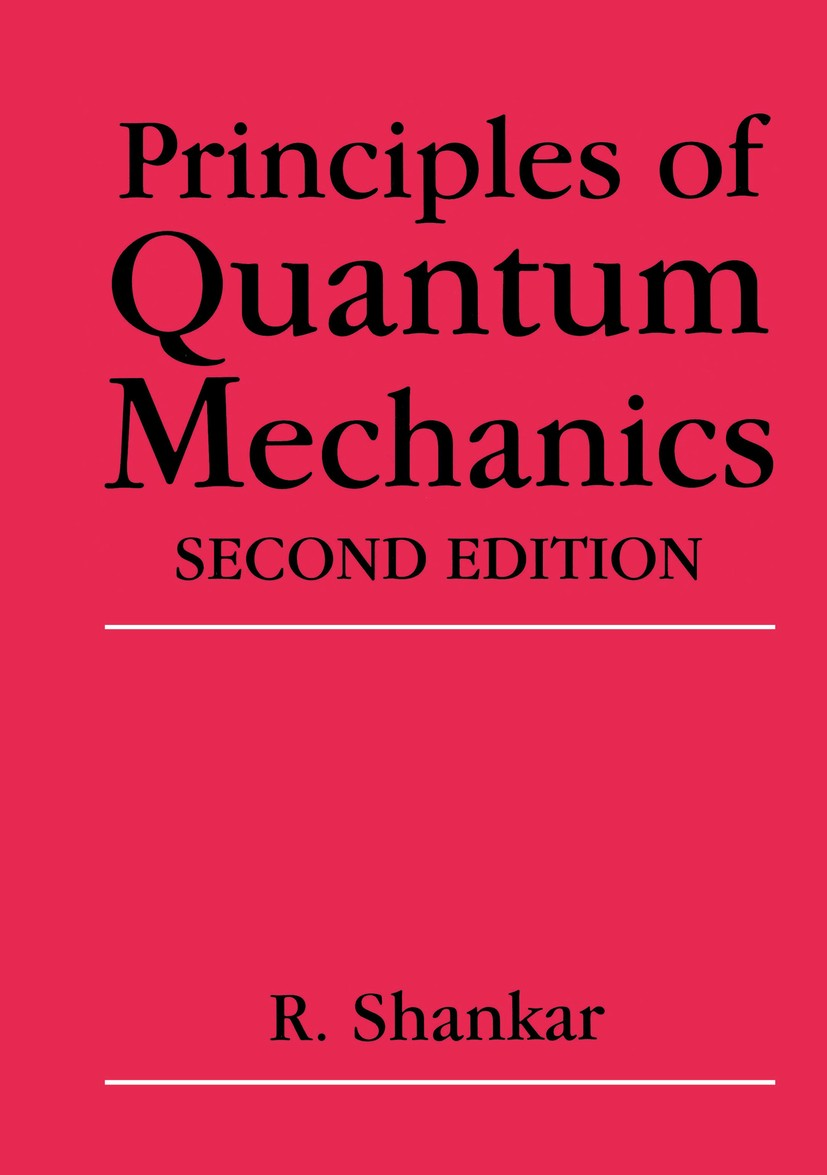
\includegraphics[width=0.8\textwidth]{images/2025-05-20-23-34-03.png}
%  \caption{}
 \end{figure} 
 \end{columns}
\end{frame}

\begin{frame}{Mechanika kwantowa}
  \begin{columns}
    \column{0.5\textwidth}
    \begin{figure}
 \centering
 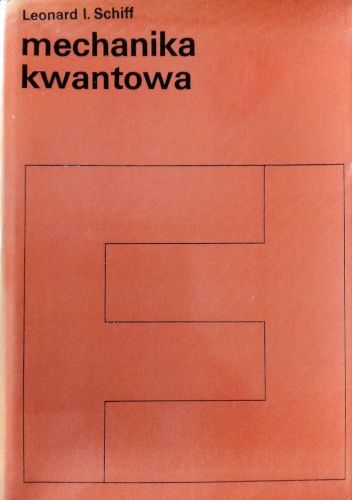
\includegraphics[width=0.8\textwidth]{images/2025-05-20-23-43-54.png}
 \caption{Biblioteka Fizyki}
 \end{figure}
 \column{0.5\textwidth}
 \begin{figure}
 \centering
 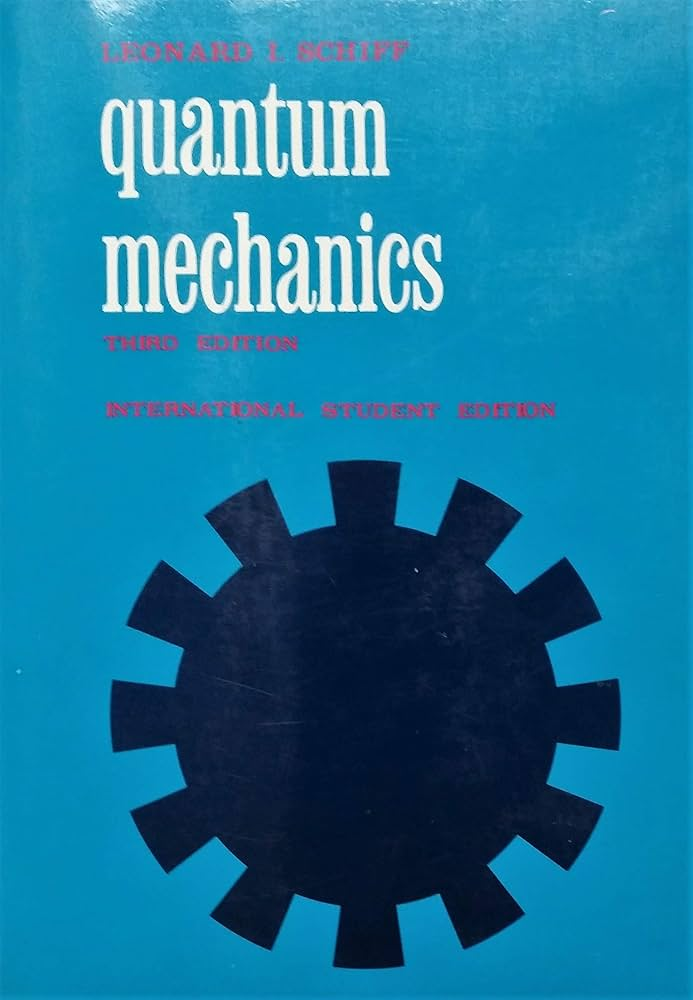
\includegraphics[width=0.8\textwidth]{images/2025-05-20-23-44-33.png}
 \caption{zembatka}
 \end{figure}
  \end{columns}
  
\end{frame}

\begin{frame}{Mechanika kwantowa}
  \begin{columns}
    \column{0.3\textwidth}
 \begin{figure}
 \centering
 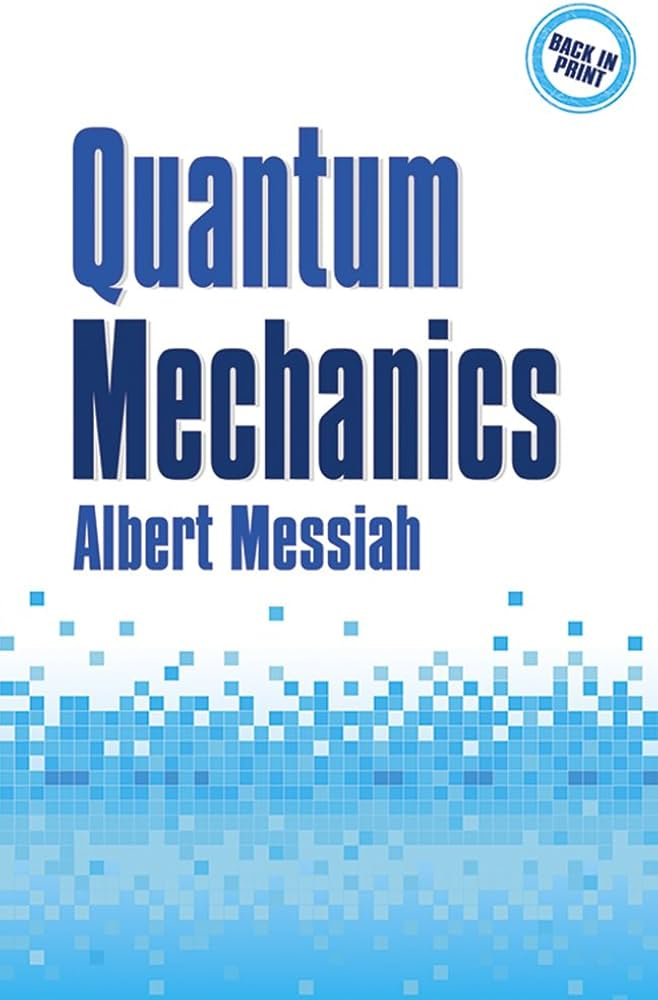
\includegraphics[width=\textwidth]{images/2025-05-20-23-32-30.png}
 \caption{Mesjasz}
 \end{figure} 
 \column{0.3\textwidth}
 \begin{figure}
 \centering
 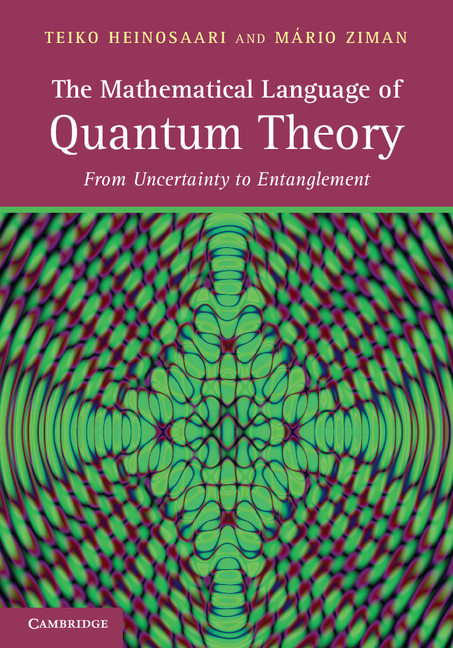
\includegraphics[width=\textwidth]{images/2025-05-20-23-38-40.png}
 \caption{Heinosaari i Zejman}
 \end{figure}
  \column{0.3\textwidth}
  \begin{figure}
 \centering
 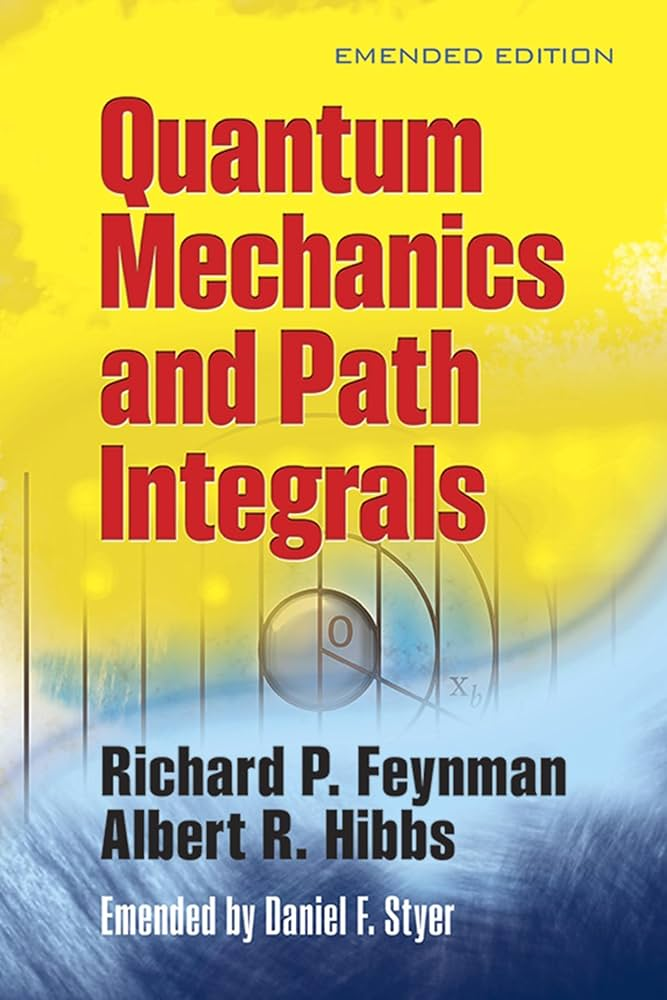
\includegraphics[width=\textwidth]{images/2025-05-20-23-39-26.png}
 \caption{Lepszy Fejnman}
 \end{figure}
 \end{columns}
\end{frame}

\subsection{Optyka}
\begin{frame}{Optyka}
\begin{columns}
  \column{0.5\textwidth}
  \begin{figure}
 \centering
 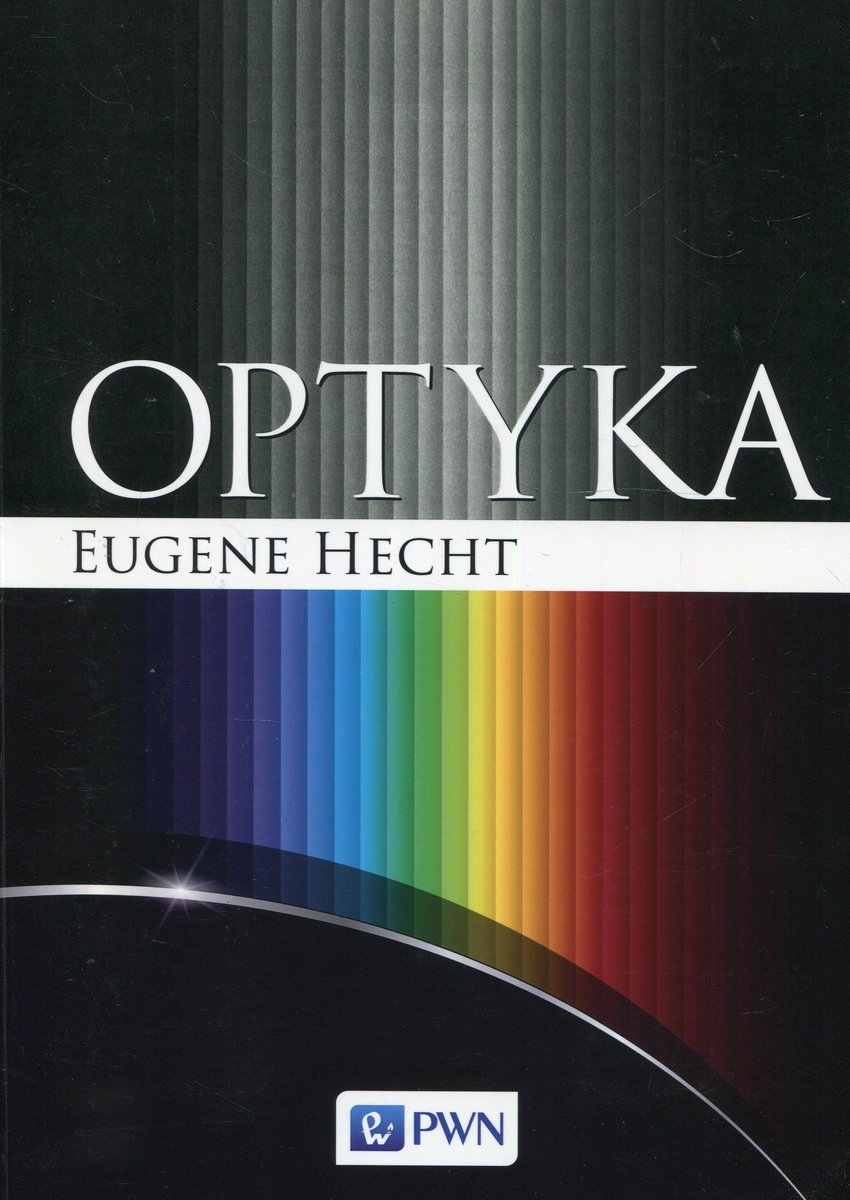
\includegraphics[width=0.8\textwidth]{images/2025-05-20-23-52-51.png}
 \caption{To trochę gejowe, nie uważacie?}
 \end{figure}
 \column{0.5\textwidth}
 \begin{figure}
 \centering
 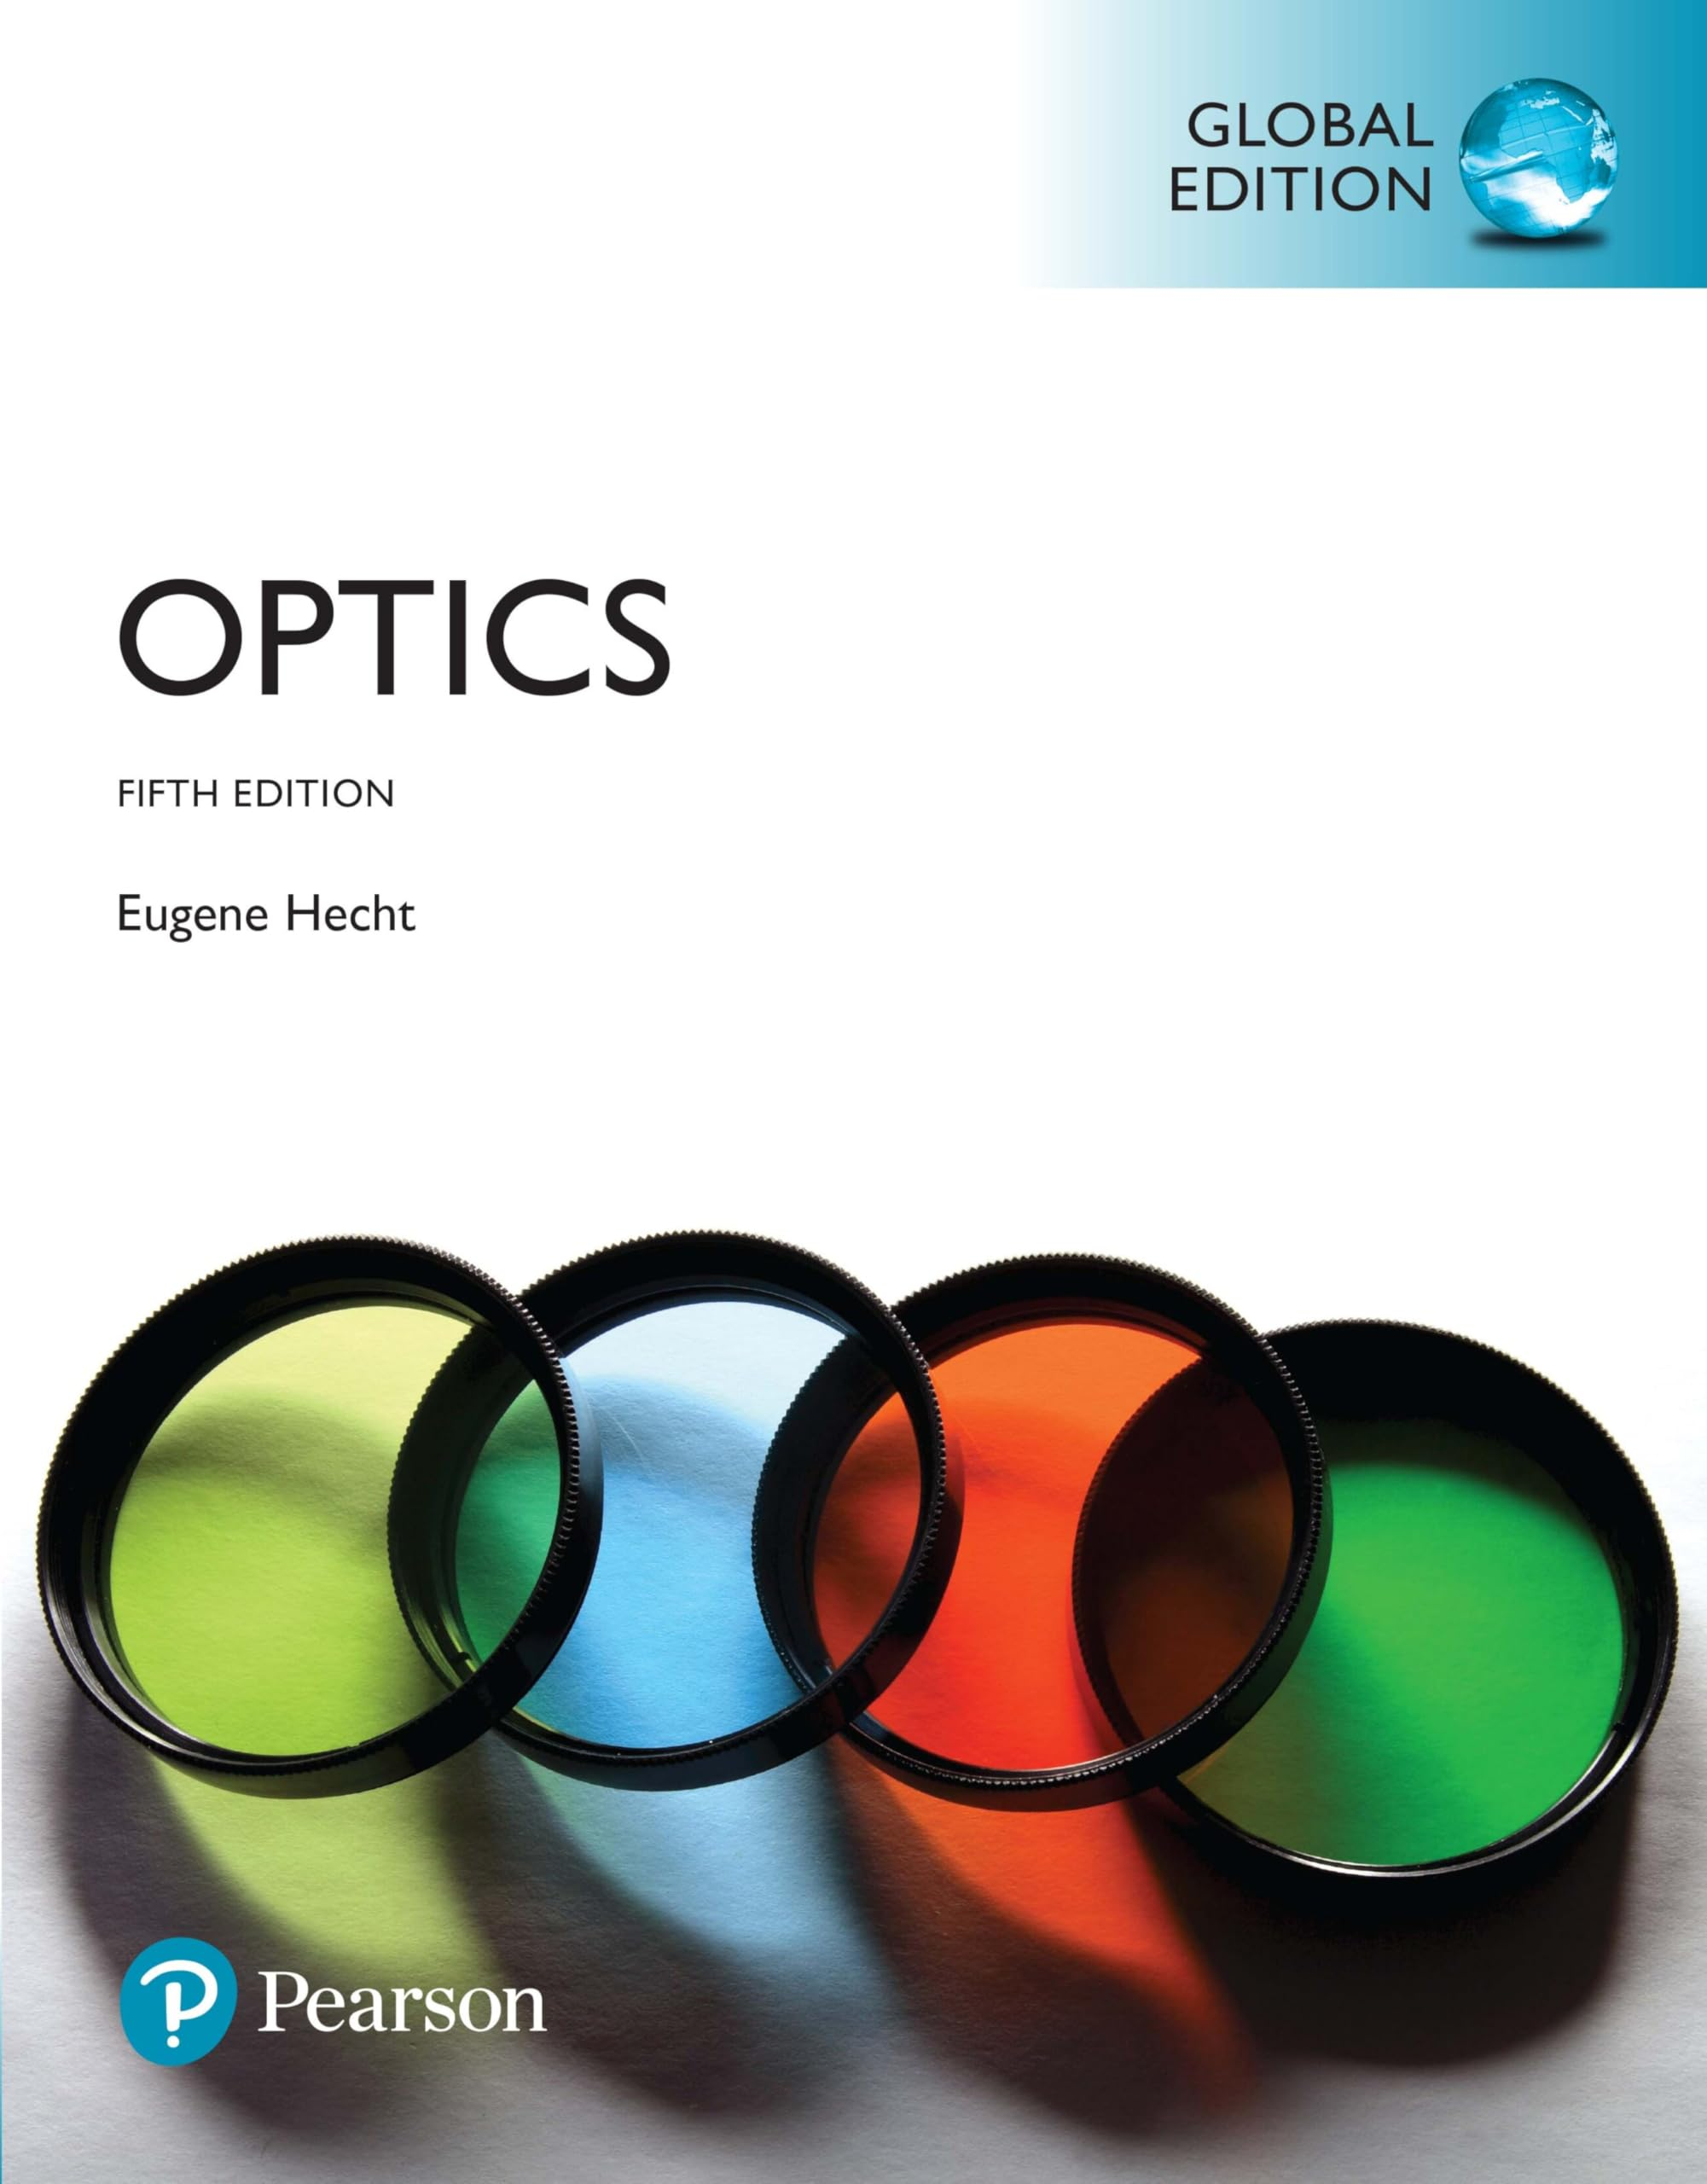
\includegraphics[width=0.8\textwidth]{images/2025-05-20-23-54-12.png}
%  \caption{}
 \end{figure}
\end{columns}

\end{frame}

\begin{frame}{Physics of light and optics \& Classical and modern optics}
  \begin{columns}
    \column{0.5\textwidth}
\begin{figure}
 \centering
 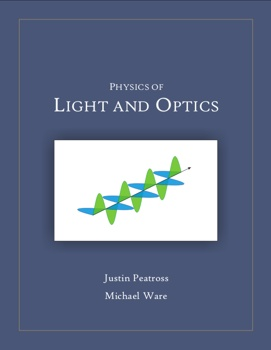
\includegraphics[width=0.8\textwidth]{images/2025-05-20-23-56-06.png}
 \caption{Made with \LaTeX{} and Julia}
 \end{figure}
 \column{0.5\textwidth}
 \begin{figure}
 \centering
 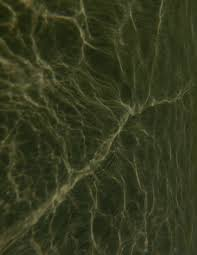
\includegraphics[width=0.8\textwidth]{images/2025-05-20-23-59-54.png}
 \caption{Made with...???}
 \end{figure}
  \end{columns}
\end{frame}

\subsection{Szczególna teoria względności}
\begin{frame}{Bibliografia Leszka M. Sokołowskiego}
\begin{columns}
  \column{0.3\textwidth}
\begin{figure}
 \centering
 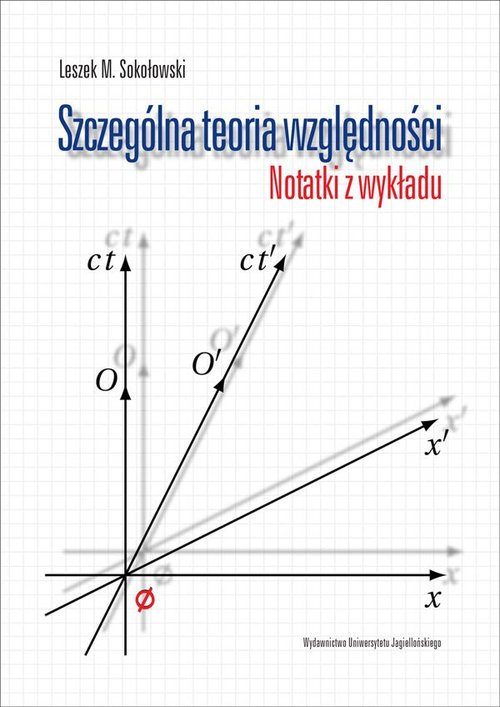
\includegraphics[width=\textwidth]{images/2025-05-21-00-14-43.png}
 \caption{Białe notatki}
 \end{figure}
 \column{0.3\textwidth}
 \begin{figure}
 \centering
 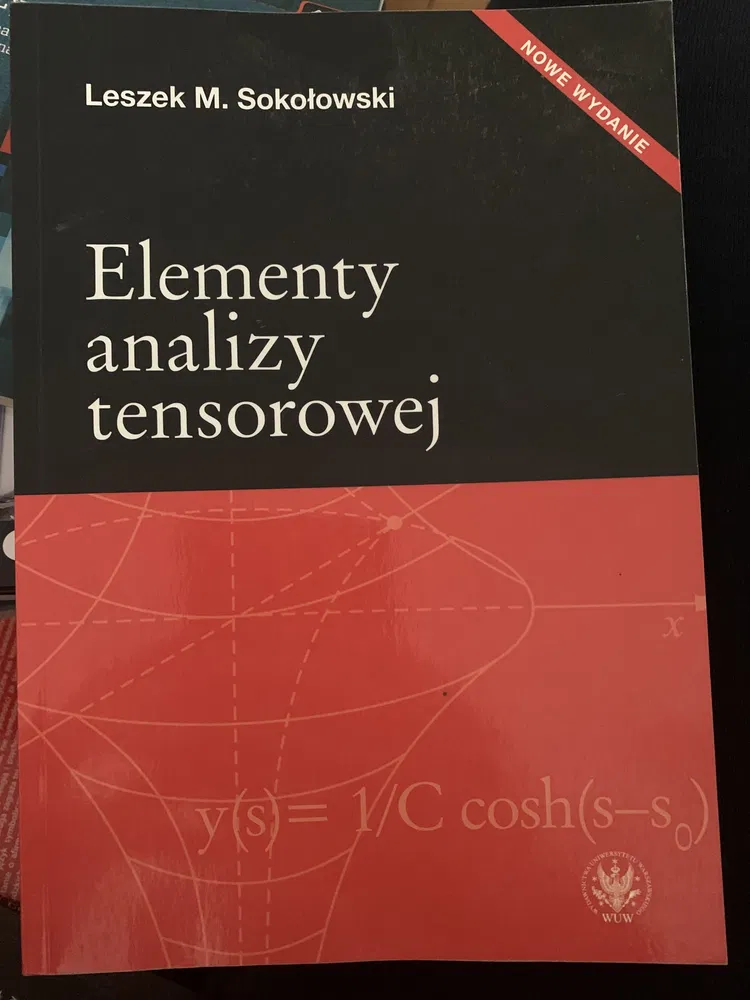
\includegraphics[width=\textwidth]{images/2025-05-21-00-07-08.png}
 \caption{Pomarańczowa książeczka}
 \end{figure}
  \column{0.3\textwidth}
\begin{figure}
 \centering
 
\includegraphics[width=\textwidth]{images/2025-05-21-00-16-10.png}
 \caption{To be continued...}
 \end{figure}
\end{columns}

\end{frame}


\section{V semestr}
\subsection{Fizyka materii skondensowanej}
\begin{frame}{Wstęp do fizyki ciała stałego}
  \begin{columns}
    \column{0.3\textwidth}
\begin{figure}
 \centering
 
\includegraphics[width=\textwidth]{images/2025-05-21-00-26-11.png}
 \caption{Zakaz używania w toalecie}
 \end{figure}
\column{0.3\textwidth}
\begin{figure}
 \centering
 
\includegraphics[width=\textwidth]{images/2025-05-21-00-26-47.png}
 \caption{(na zajęciach zresztą też)}
 \end{figure}
 \column{0.3\textwidth}
 \begin{figure}
 \centering
 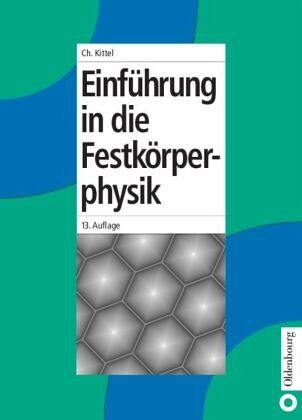
\includegraphics[width=\textwidth]{images/2025-05-21-14-38-56.png}
 \caption{}
 \end{figure}
 \end{columns}
\end{frame}

\begin{frame}{Fizyka ciała stałego}
  \begin{columns}
    \column{0.3\textwidth}
\begin{figure}
 \centering
 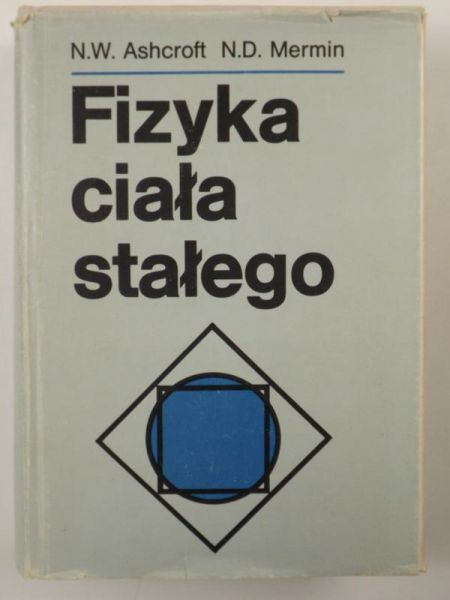
\includegraphics[width=\textwidth]{images/2025-05-21-00-30-48.png}
%  \caption{}
 \end{figure}
\column{0.3\textwidth}
\begin{figure}
 \centering
 
\includegraphics[width=\textwidth]{images/2025-05-21-00-30-10.png}
%  \caption{}
 \end{figure}
 \column{0.3\textwidth}
 \begin{figure}
 \centering
 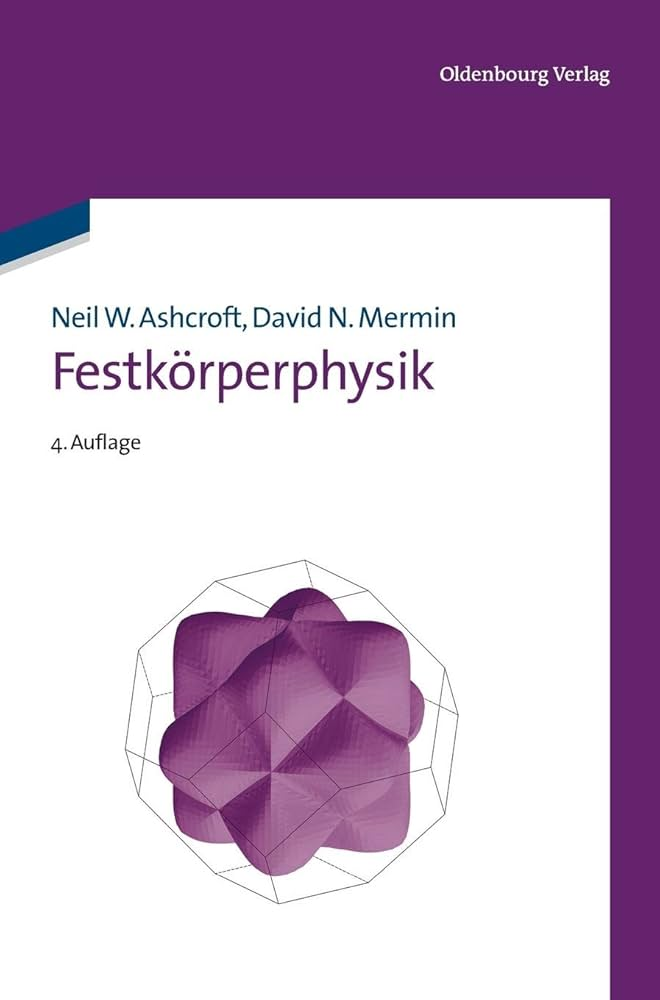
\includegraphics[width=\textwidth]{images/2025-05-21-00-31-25.png}
%  \caption{}
 \end{figure}
 \end{columns}
\end{frame}

\begin{frame}{Fizyka ciała stałego}
  \begin{columns}
    \column{0.3\textwidth}
\begin{figure}
 \centering
 
\includegraphics[width=\textwidth]{images/2025-05-21-00-33-12.png}
%  \caption{}
 \end{figure}
\column{0.3\textwidth}
\begin{figure}
 \centering
 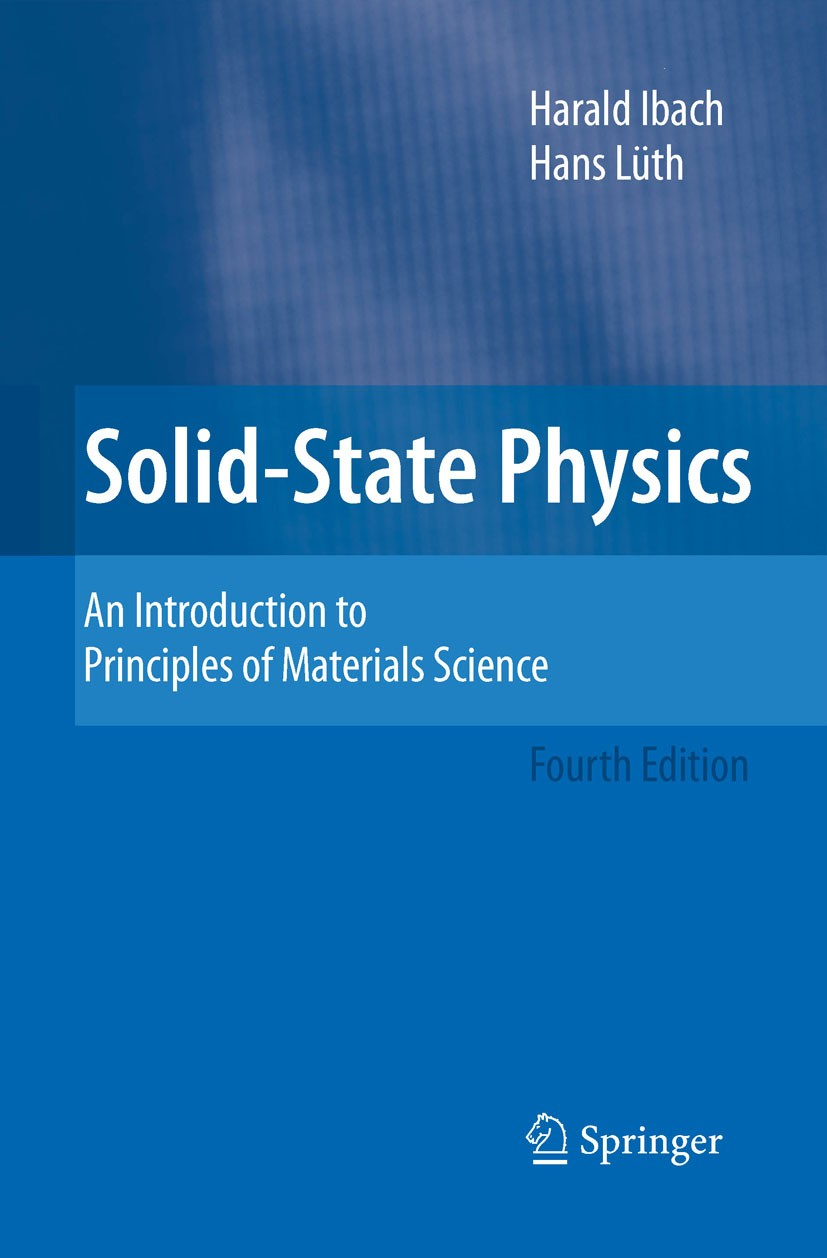
\includegraphics[width=\textwidth]{images/2025-05-21-00-33-28.png}
%  \caption{}
 \end{figure}
 \column{0.3\textwidth}
 \begin{figure}
 \centering
 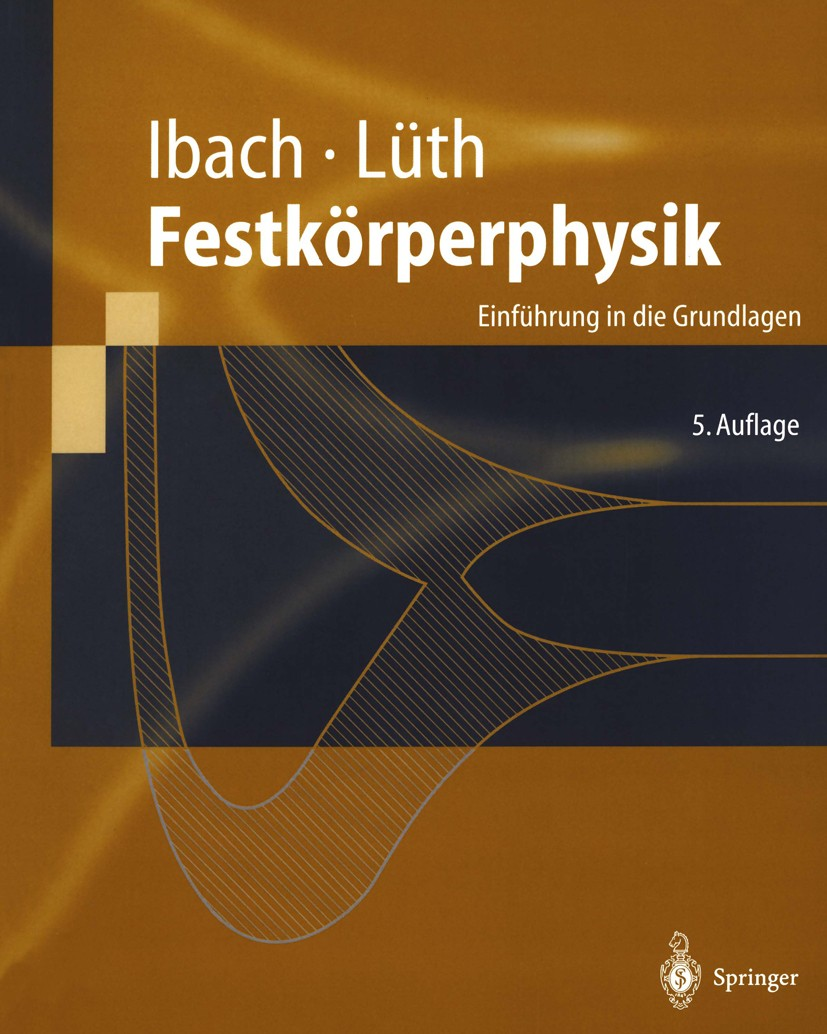
\includegraphics[width=\textwidth]{images/2025-05-21-00-34-03.png}
%  \caption{}
 \end{figure}
 \end{columns}
\end{frame}


\subsection{Elektrodynamika klasyczna}
\begin{frame}{Elektrodynamika klasyczna}
  \begin{columns}
    \column{0.25\textwidth}
\begin{figure}
 \centering
 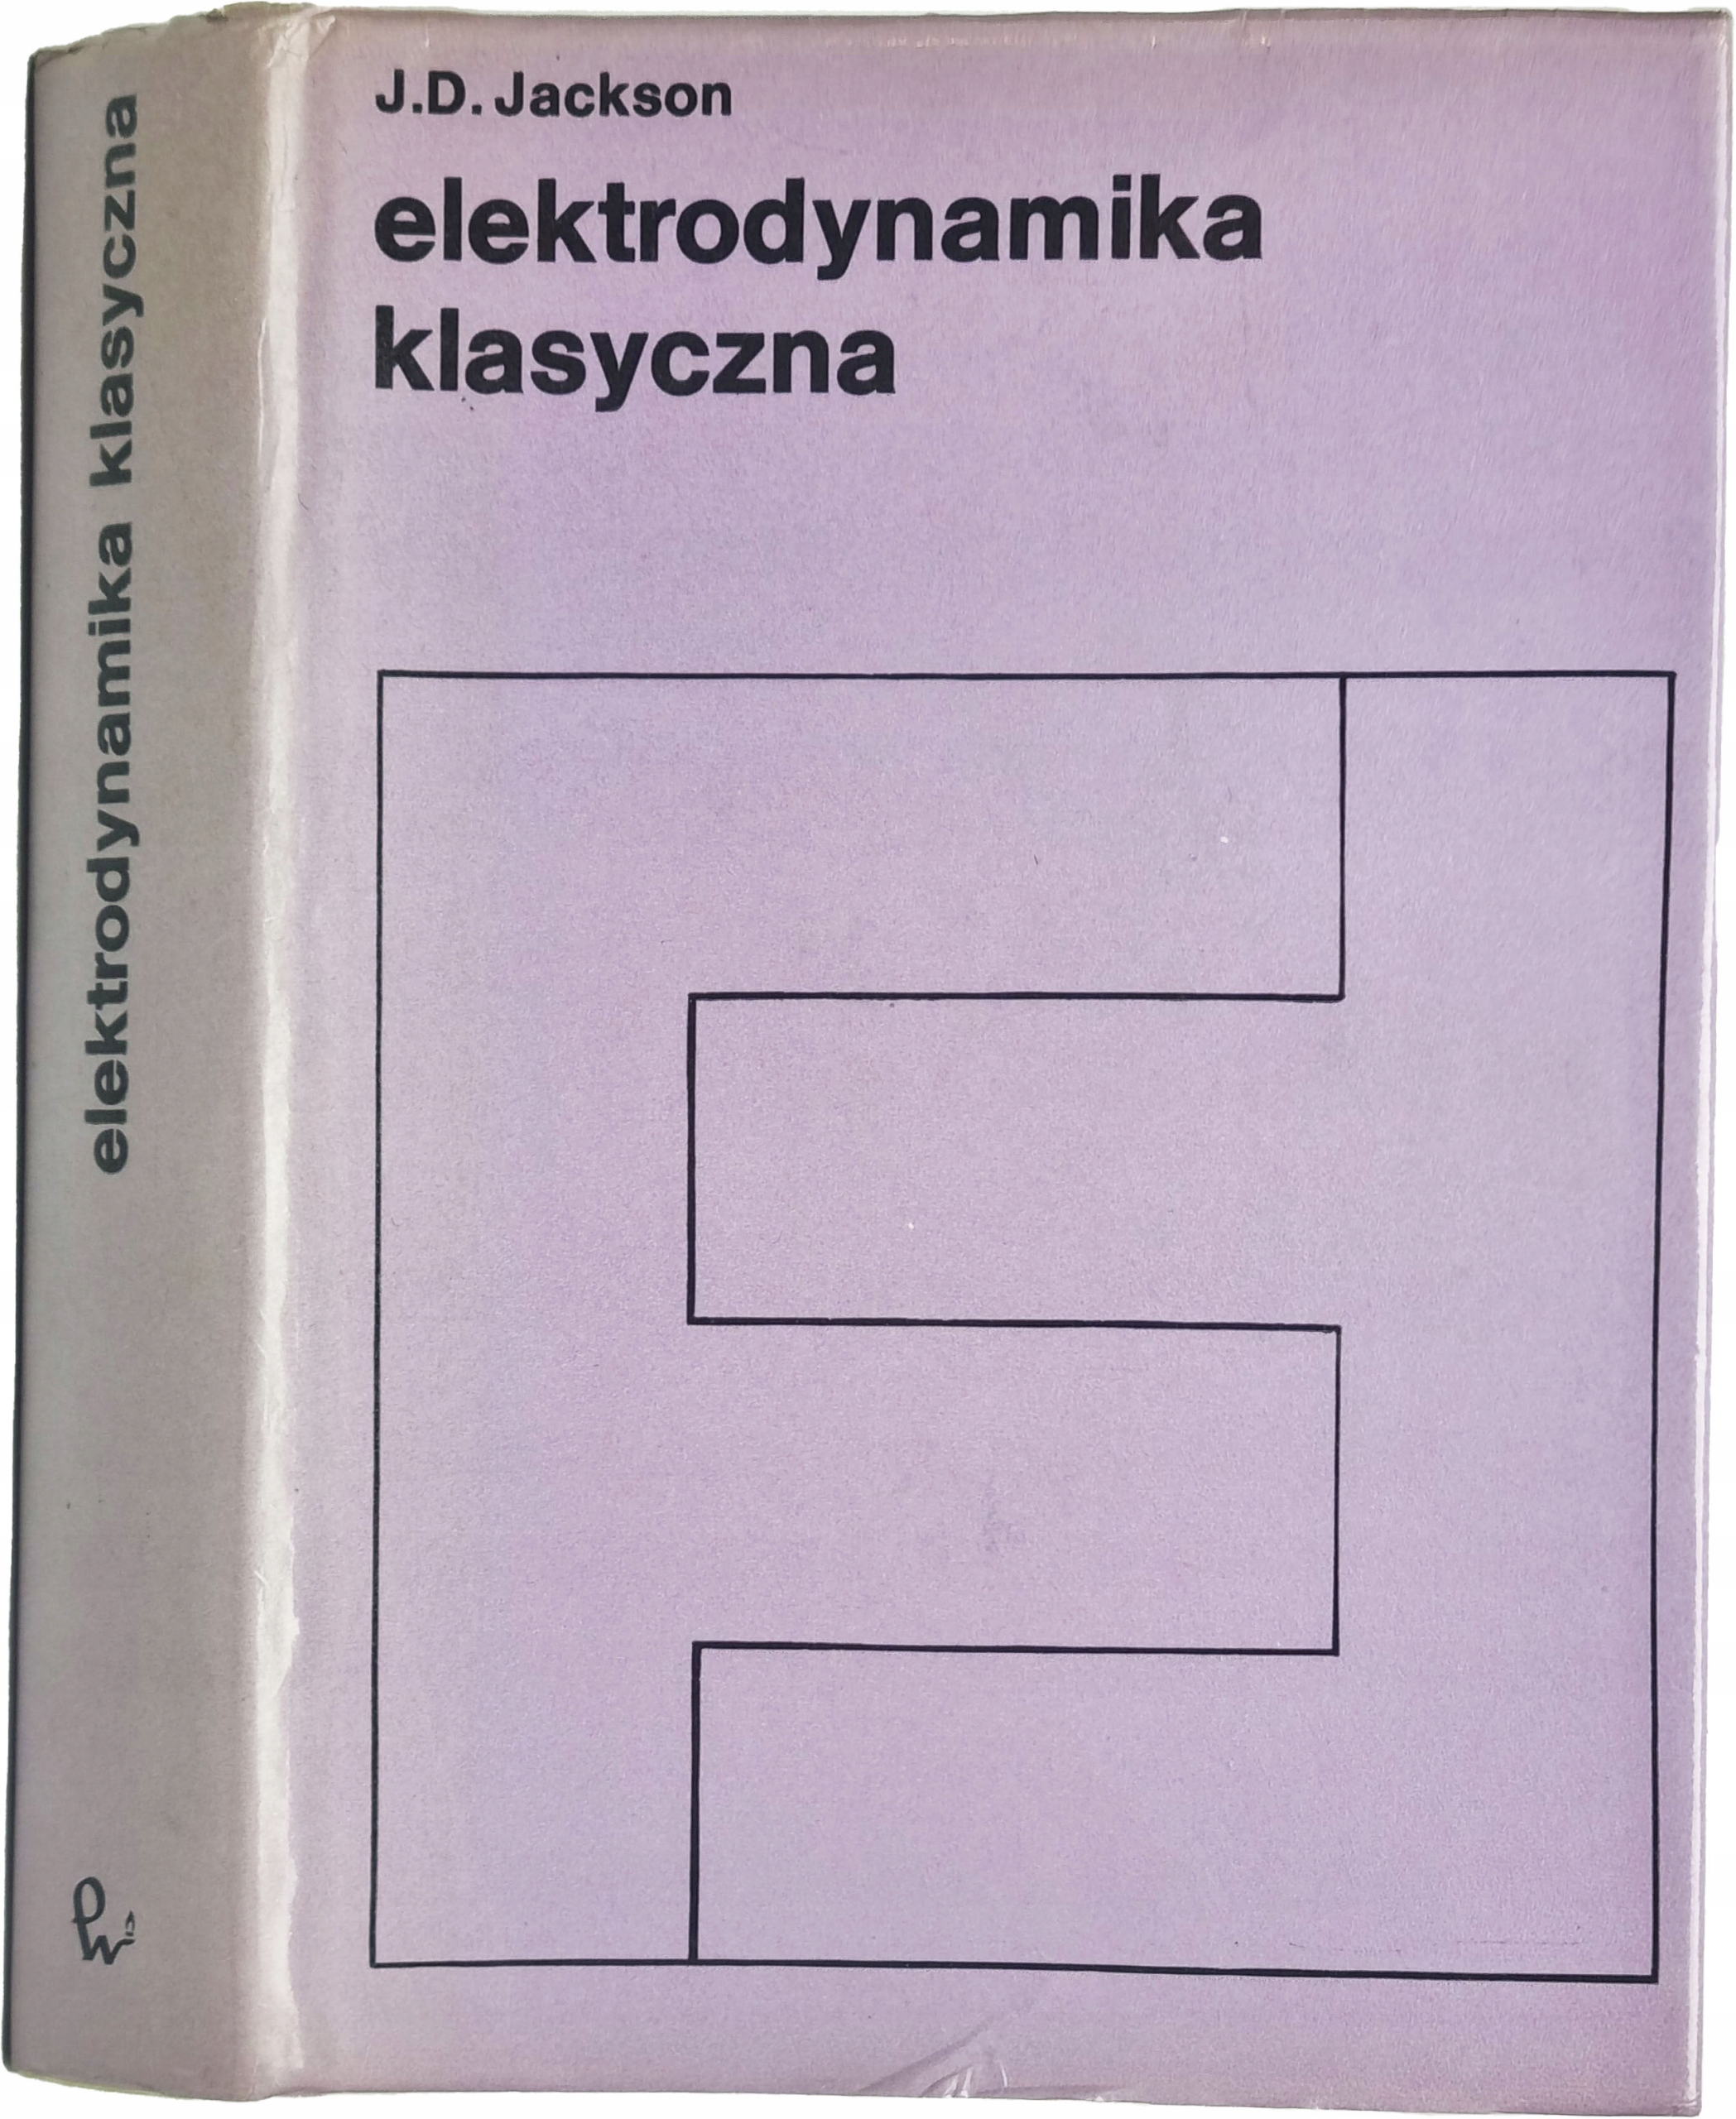
\includegraphics[width=0.95\textwidth]{images/2025-05-21-00-51-49.png}
%  \caption{}
 \end{figure}
    \column{0.25\textwidth}
 \begin{figure}
 \centering
 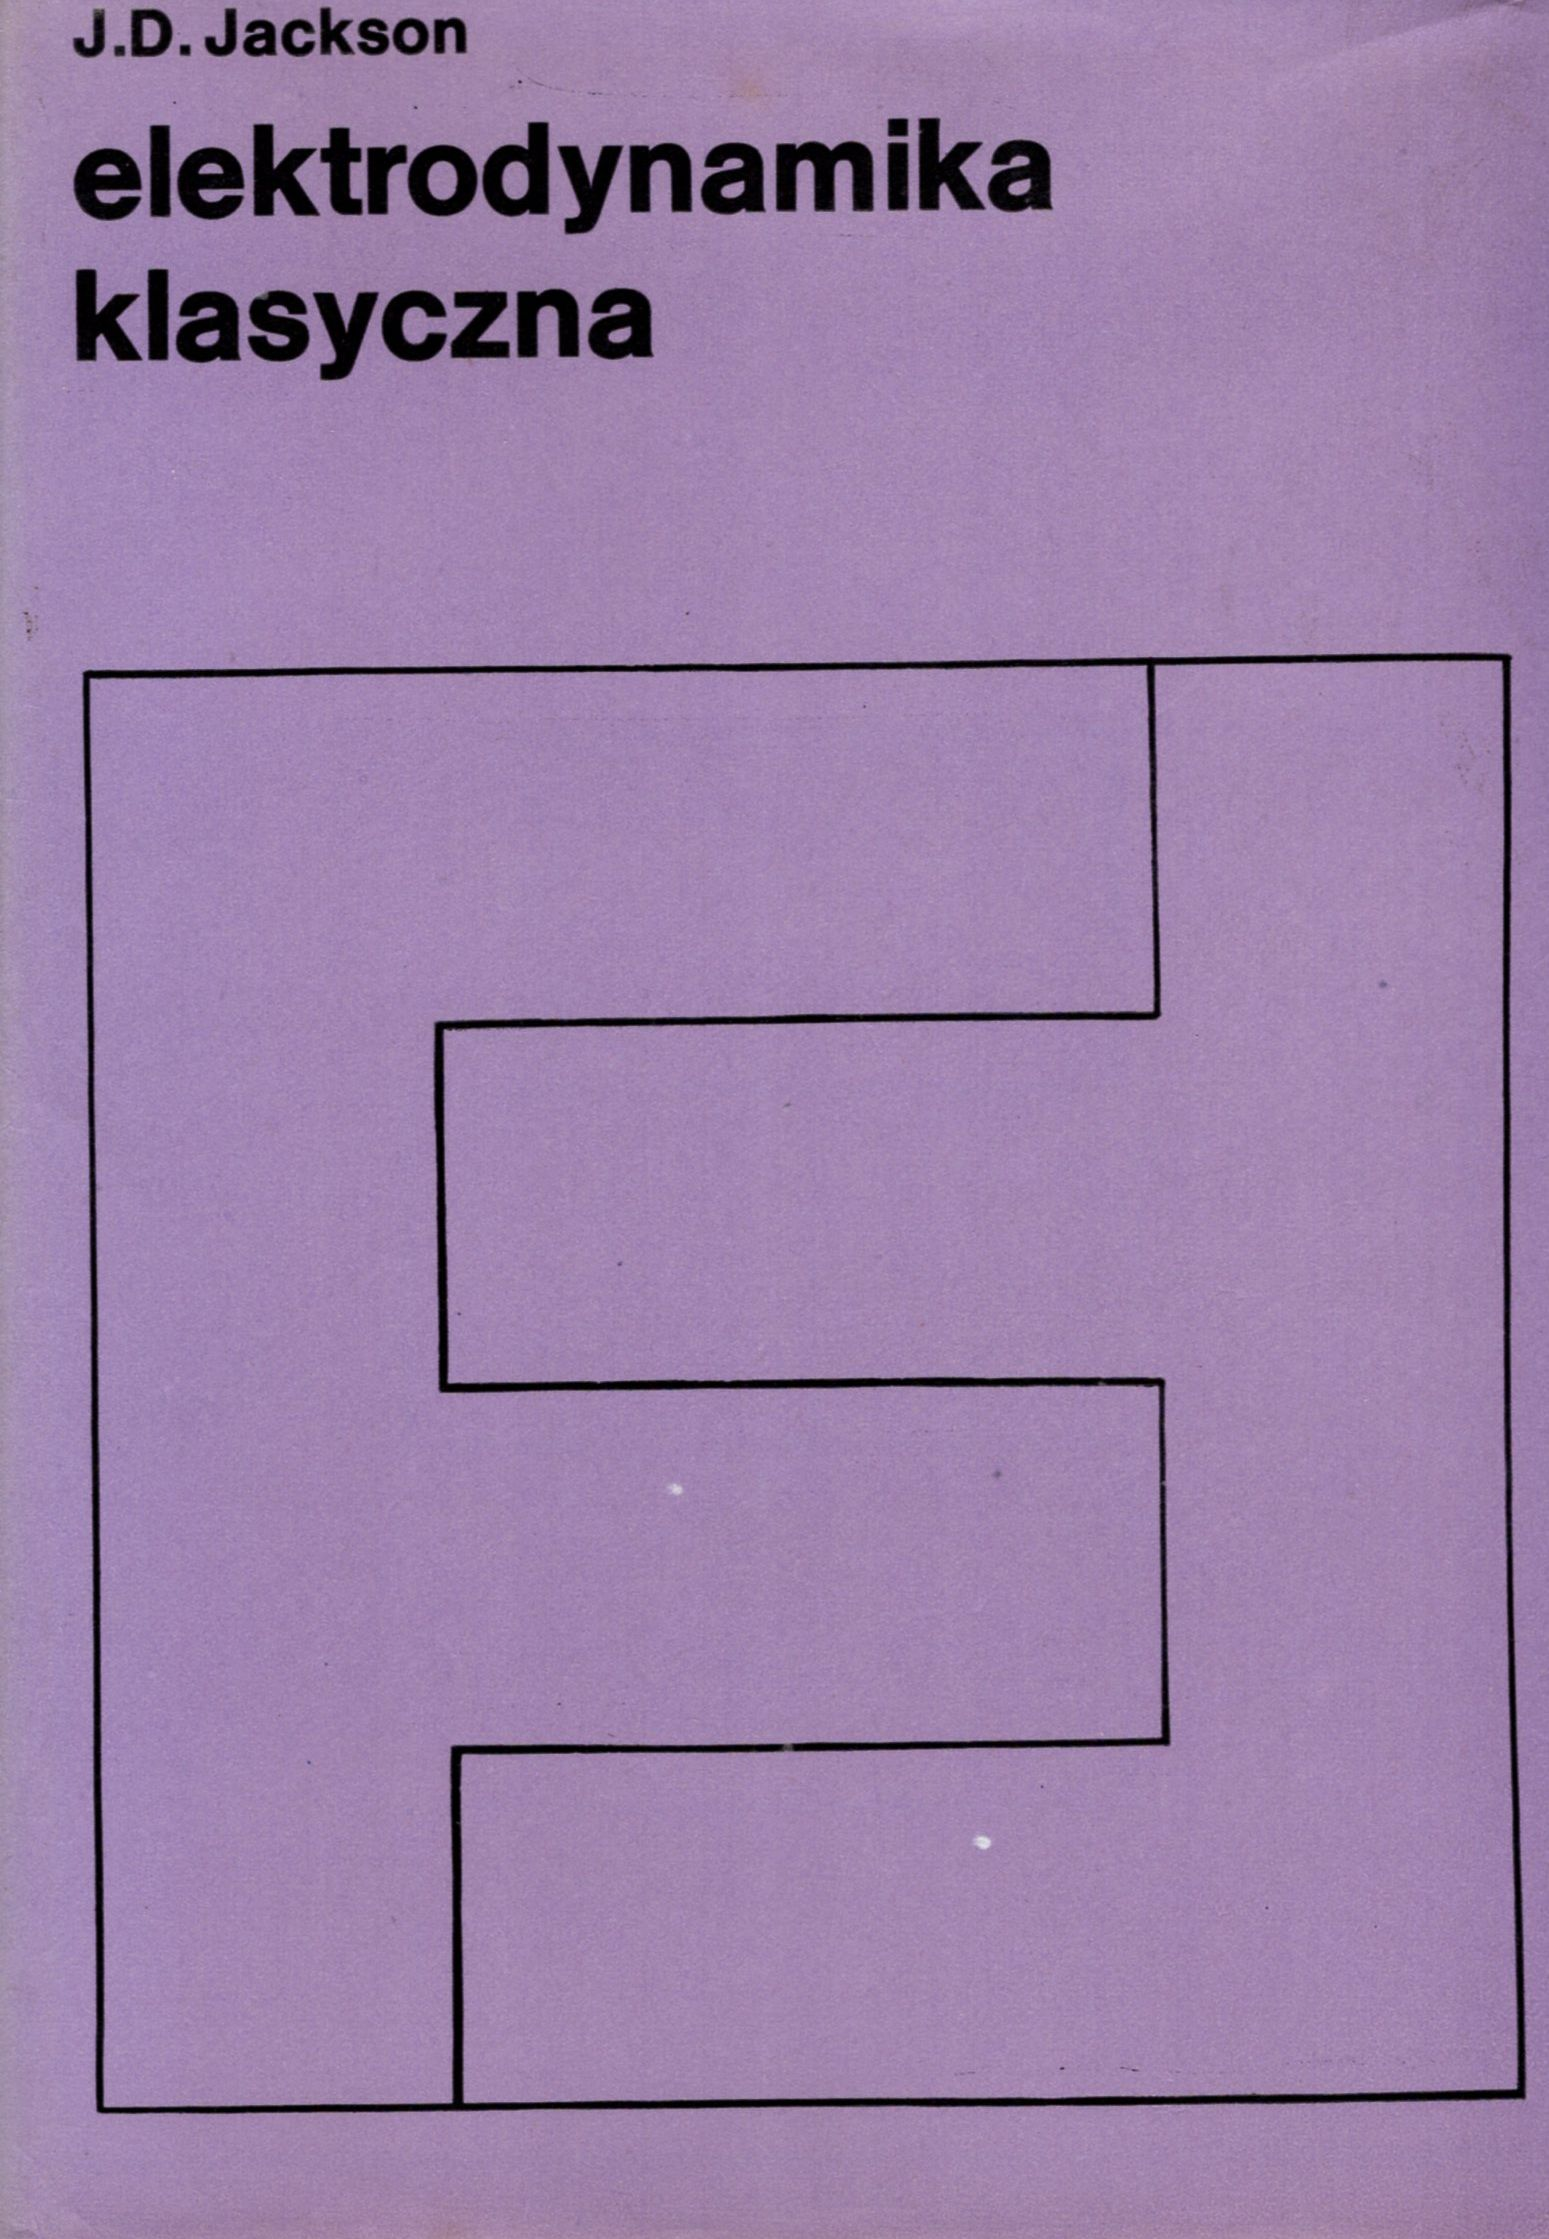
\includegraphics[width=0.95\textwidth]{images/2025-05-21-00-52-28.png}
%  \caption{}
 \end{figure}
 \column{0.25\textwidth}
 \begin{figure}
 \centering
 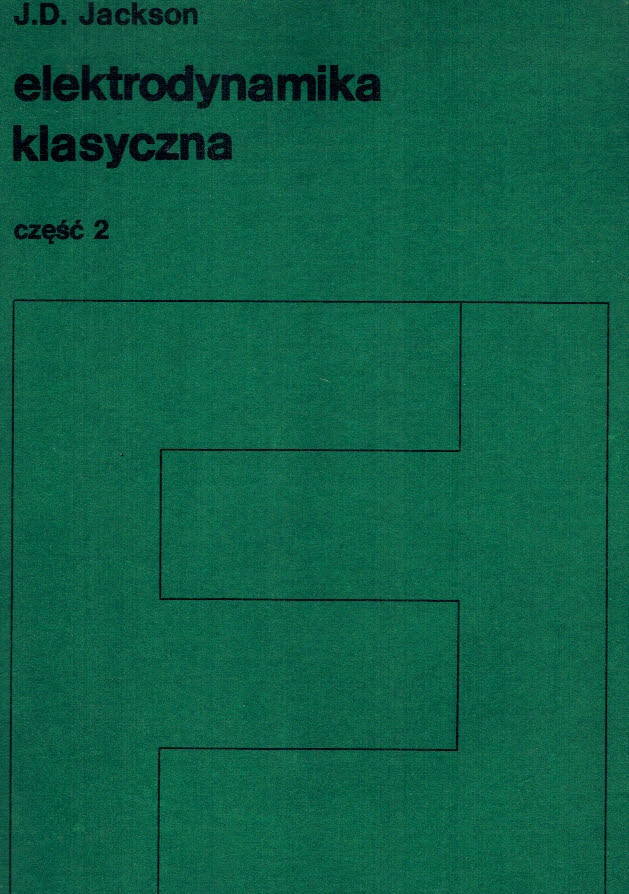
\includegraphics[width=0.95\textwidth]{images/2025-05-21-00-52-08.png}
%  \caption{}
 \end{figure}
    \column{0.25\textwidth}
\begin{figure}
 \centering
 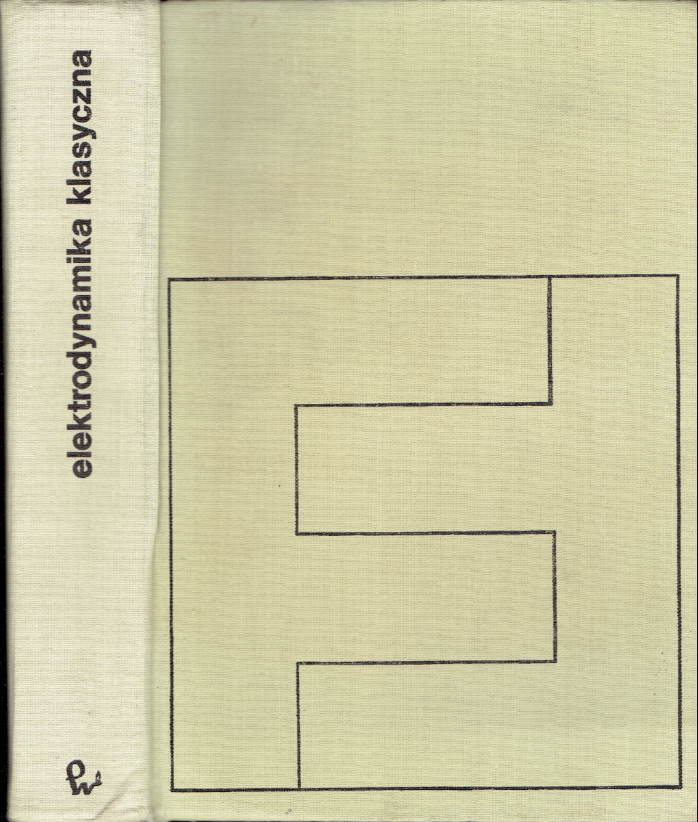
\includegraphics[width=0.95\textwidth]{images/2025-05-21-01-06-23.png}
%  \caption{}
 \end{figure}

 \end{columns}
\end{frame}

\begin{frame}{Elektrodynamika klasyczna}
  \begin{columns}
    \column{0.25\textwidth}
\begin{figure}
 \centering
 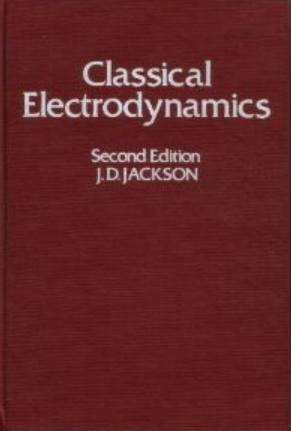
\includegraphics[width=0.95\textwidth]{images/2025-05-21-01-08-27.png}
%  \caption{}
 \end{figure}
    \column{0.25\textwidth}
\begin{figure}
 \centering
 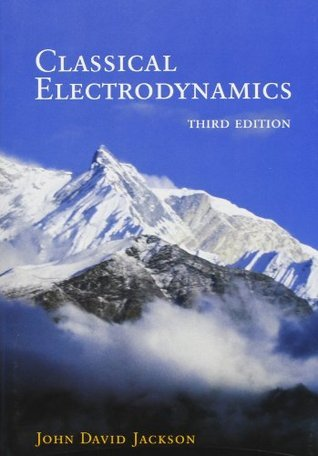
\includegraphics[width=0.95\textwidth]{images/2025-05-21-01-08-39.png}
%  \caption{}
 \end{figure}
 \column{0.25\textwidth}
\begin{figure}
 \centering
 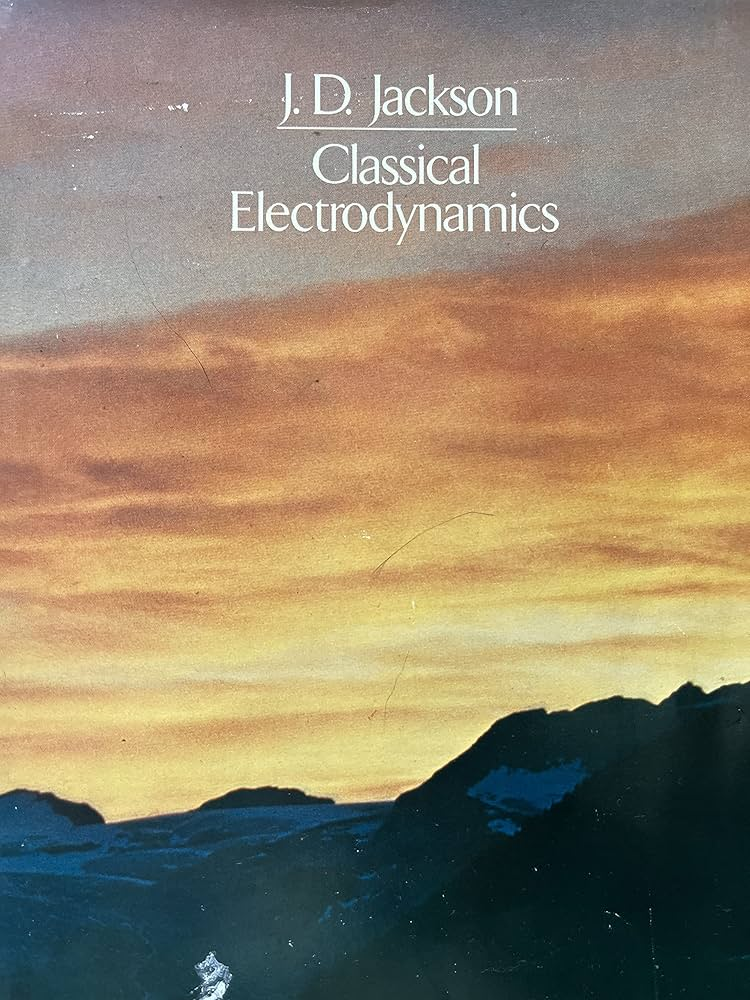
\includegraphics[width=0.95\textwidth]{images/2025-05-21-01-08-51.png}
%  \caption{}
 \end{figure}
    \column{0.25\textwidth}
\begin{figure}
 \centering
 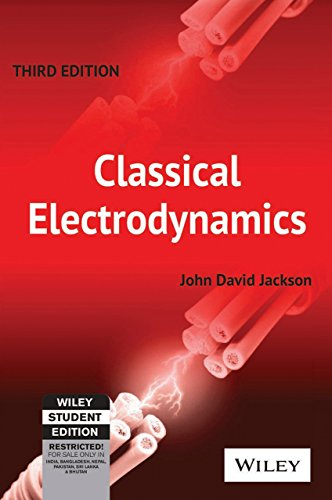
\includegraphics[width=0.95\textwidth]{images/2025-05-21-01-09-08.png}
%  \caption{}
 \end{figure}
 \end{columns}
\end{frame}

\section{VI semestr}
\subsection{Fizyka statystyczna}
\begin{frame}{Huangi}
  \begin{columns}
    \column{0.5\textwidth}
\begin{figure}
 \centering
 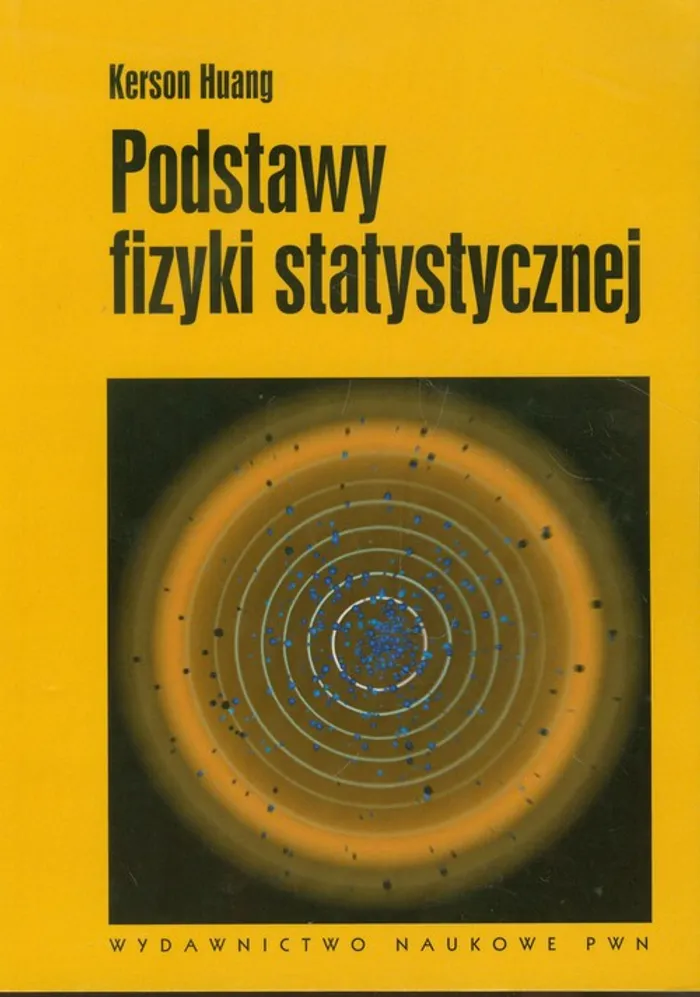
\includegraphics[width=0.8\textwidth]{images/2025-05-21-01-12-26.png}
 \caption{mały Huang}
 \end{figure}
 \column{0.5\textwidth}
 \begin{figure}
 \centering
 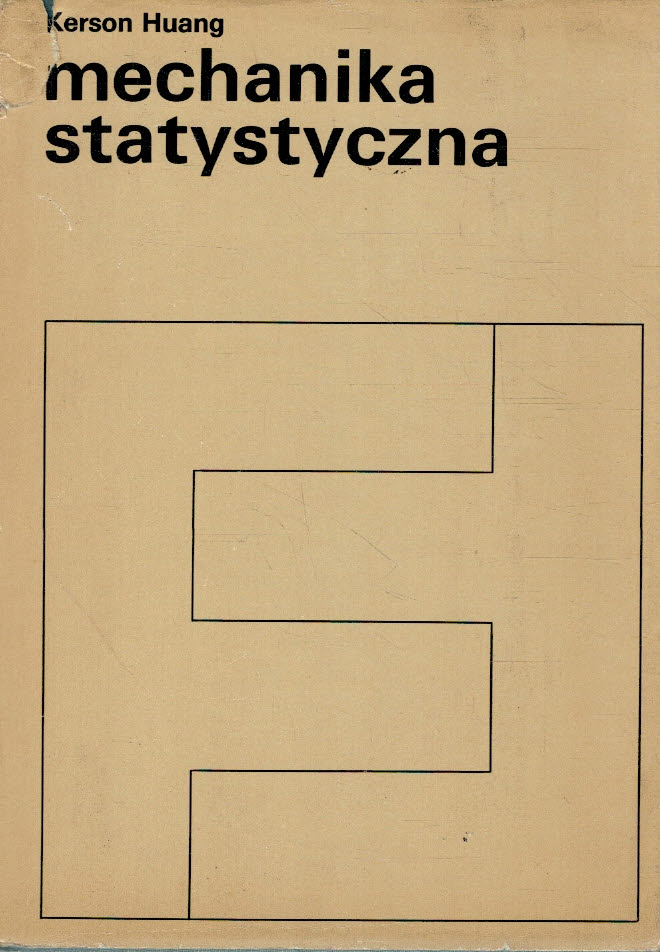
\includegraphics[width=0.8\textwidth]{images/2025-05-21-02-33-18.png}
 \caption{duży Huang}
 \end{figure}

 \end{columns}
\end{frame}


\subsection{Fizyka cząstek elementarnych}

\begin{frame}{Cząstki}
  \begin{columns}
    \column{0.3\textwidth}
    \begin{figure}
 \centering
 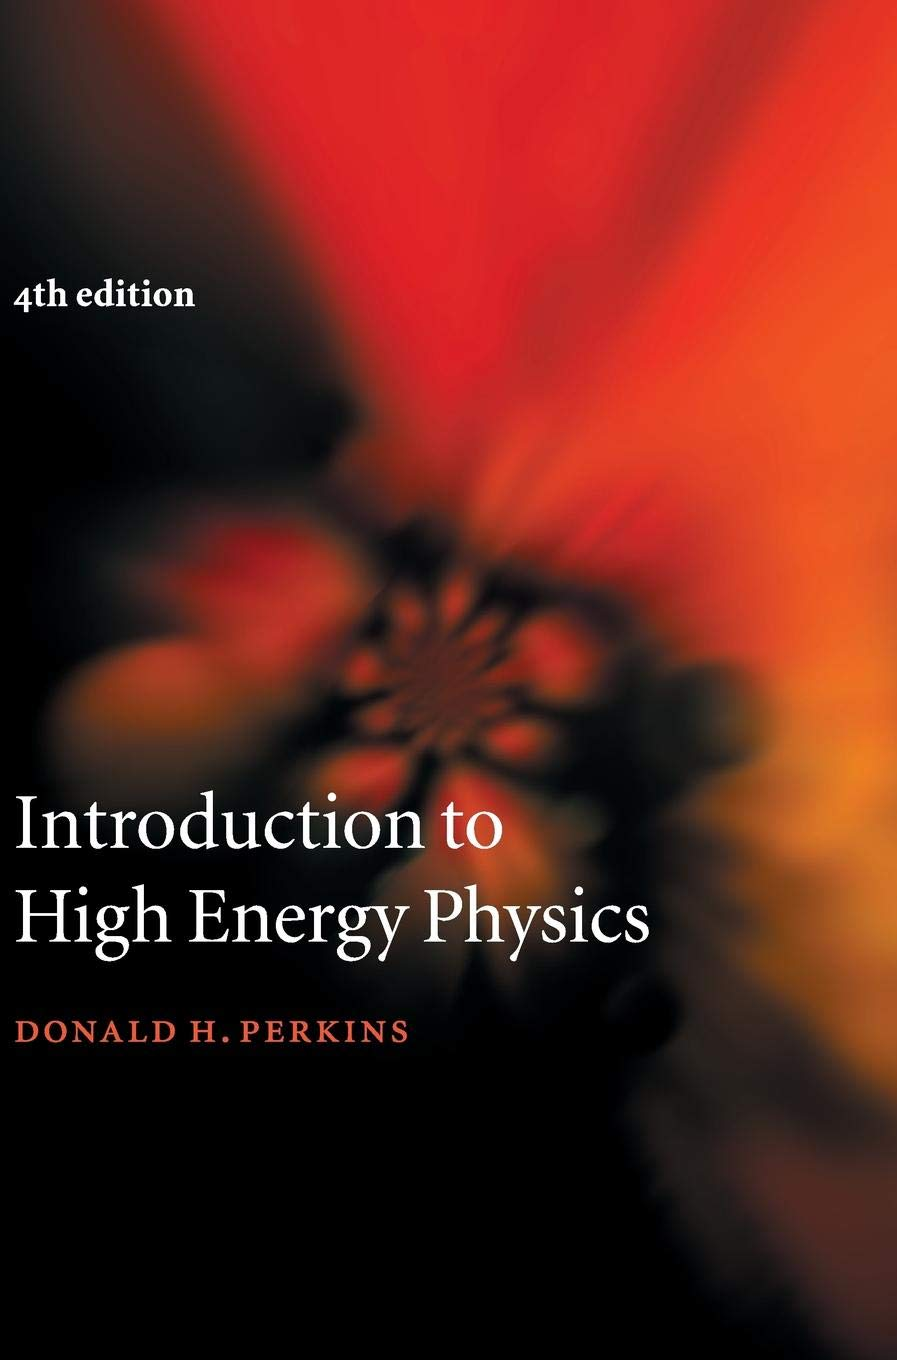
\includegraphics[width=\textwidth]{images/2025-05-21-13-22-03.png}
 \caption{Perkins (też po polsku)}
 \end{figure}
    \column{0.3\textwidth}
    \begin{figure}
 \centering
 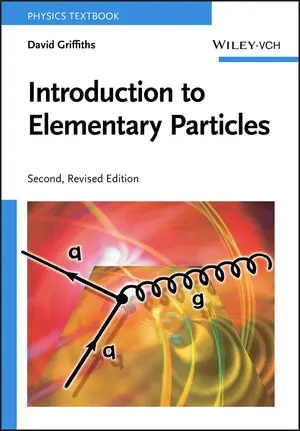
\includegraphics[width=\textwidth]{images/2025-05-21-13-18-27.png}
 \caption{Griffiths (tak, ten)}
 \end{figure}
  \column{0.3\textwidth}
  \begin{figure}
 \centering
 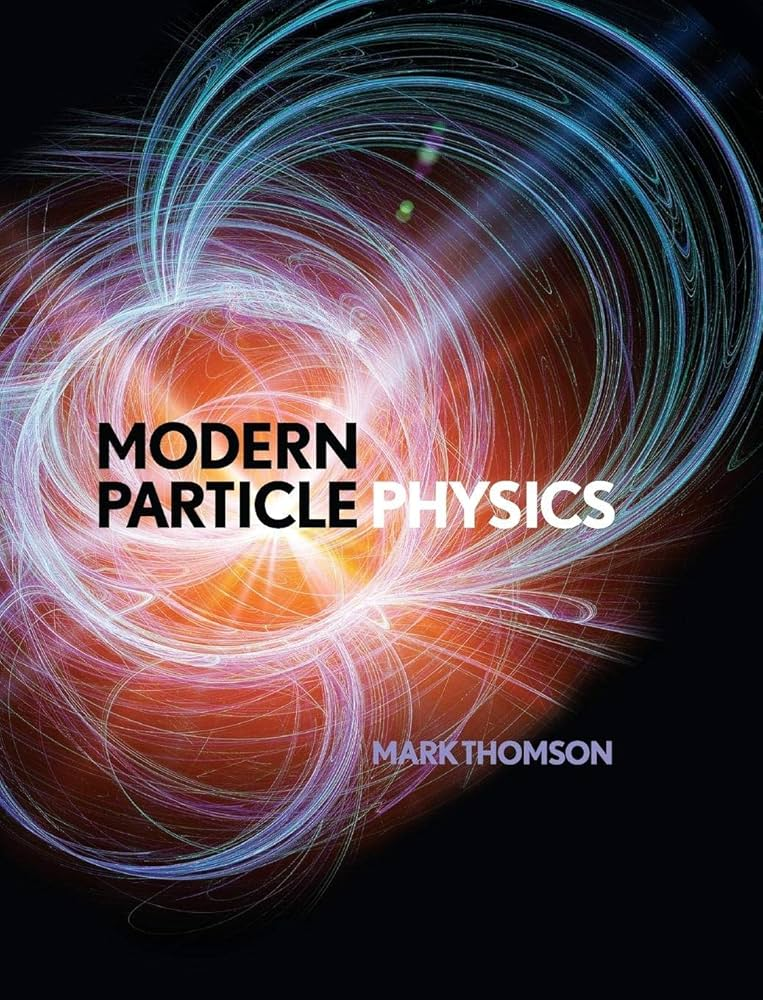
\includegraphics[width=\textwidth]{images/2025-05-21-13-19-22.png}
 \caption{Thomson}
 \end{figure}
\end{columns}
\end{frame}
\begin{frame}{Inne cząstki}
  \begin{columns}
    \column{0.3\textwidth}
\begin{figure}
 \centering
 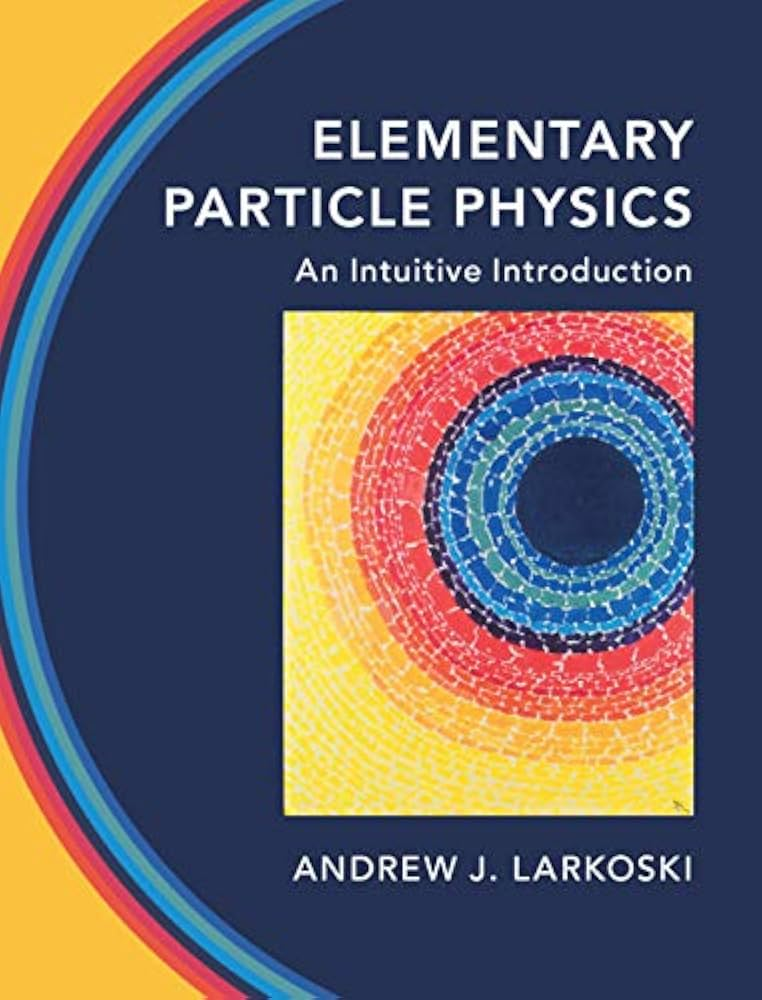
\includegraphics[width=\textwidth]{images/2025-05-21-02-29-44.png}
 \caption{Larkoski}
 \end{figure}
 \column{0.3\textwidth}
 \begin{figure}
 \centering
 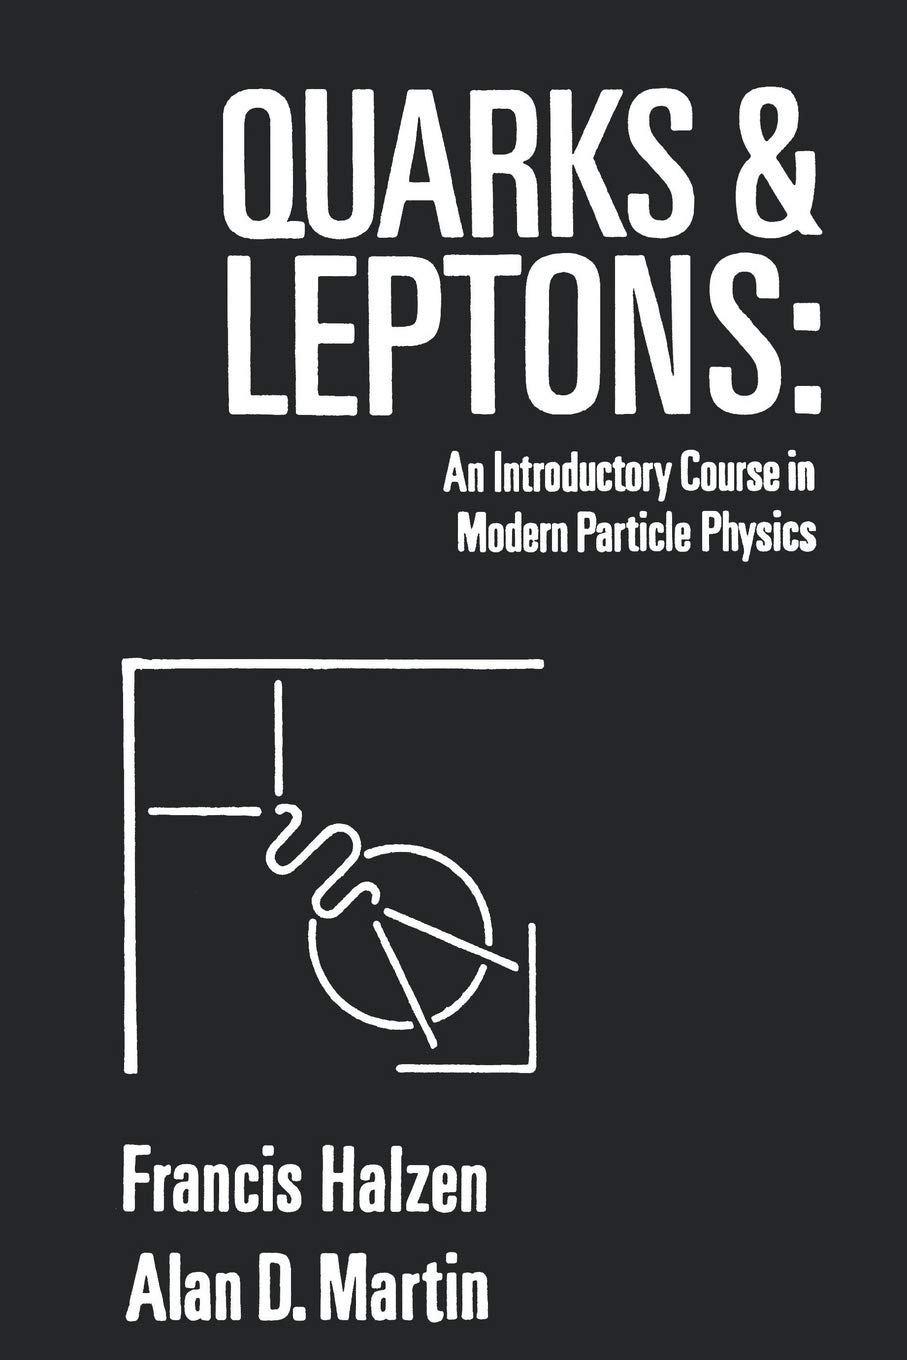
\includegraphics[width=\textwidth]{images/2025-05-21-02-30-34.png}
 \caption{Halzen\&Martin}
 \end{figure}
 \column{0.3\textwidth}
 \begin{figure}
 \centering
 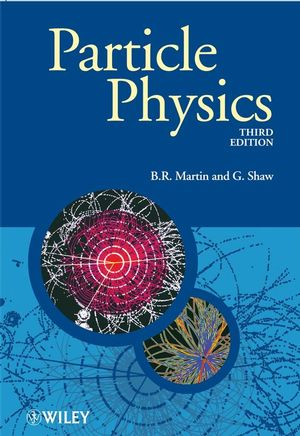
\includegraphics[width=\textwidth]{images/2025-05-21-02-31-13.png}
 \caption{Martin\&Shaw}
 \end{figure}

 \end{columns}
\end{frame}


\section*{}
\begin{frame}{Wolne wnioski}{}
  
\end{frame}


\begin{frame}{}{}
  \vspace{-1.5cm}
\begin{figure}
\centering
  \begin{tikzpicture}
    \duck[parrot, body=gray!30!yellow, head=gray!30!yellow, bill=red, torch=gray!70!brown, tshirt=blue!10!black, ribbon=gray, bowtie=blue!50!white, crazyhair=black]
    %\addwater{blue!50!cyan}
    \fill[cyan!20!white] (-1.4,1.8) ellipse (1.8 and 0.5);
\fill[cyan!20!white] (-0.2,1.54) -- (0.2,1.35) -- (0.0,1.6) -- cycle;
\node at (-1.4,1.8) {dziękuję za uwagę};
  \end{tikzpicture}
  \end{figure}


  
  \begin{figure}
  \centering
        % 
\includegraphics[height=0.3\linewidth]{images/2025-05-13-15-25-41.png}\\
      \qrcode[height=0.3\textwidth]{https://github.com/falcotinnunculus/przezrocza/blob/wladca/twink/main.pdf}
  {\tiny \url{https://github.com/falcotinnunculus/przezrocza/blob/wladca/twink/main.pdf}}

  \end{figure}
\vspace{-4.25cm}
\transparent{0.7}
  \begin{figure}
      \centering
      % \caption{Caption}
      % \label{fig:enter-label}
  \end{figure}
\end{frame}


% \end{document}

 \end{document}